\documentclass[12pt]{ucthesis}

\usepackage{etex}
\usepackage[morefloats=125]{morefloats}
\usepackage[hyphens]{url}
\usepackage[breaklinks=true]{hyperref}
\usepackage{subfig}
\usepackage{graphicx}
\graphicspath{ {figures/} }
\usepackage{tabularx}
\usepackage{amssymb}
\usepackage{amsmath}
\usepackage[letterpaper]{geometry}
\usepackage[overload]{textcase}
\usepackage{color}
\usepackage[nonumberlist,toc]{glossaries}
\usepackage{wrapfig}
\usepackage{longtable}
\usepackage{morefloats}
\usepackage{float}
\usepackage{listings}
\usepackage{makecell}
\usepackage[titletoc]{appendix}
\usepackage{cleveref}
\usepackage[]{algorithm2e}

\makeindex
\makeglossaries

\bibliographystyle{abbrv}

\setlength{\parindent}{0.25in} \setlength{\parskip}{6pt}
\geometry{verbose,nohead,tmargin=1in,bmargin=1in,lmargin=1.5in,rmargin=1in}
\setcounter{tocdepth}{2}

% Different font in captions (single-spaced, bold) ------------
\newcommand{\captionfonts}{\small\bf\ssp}

\newcommand{\mycaption}[2]{\caption[#1 --- #2]{#1 --- #2}}

\makeatletter  % Allow the use of @ in command names
\long\def\@makecaption#1#2{%
  \vskip\abovecaptionskip
  \sbox\@tempboxa{{\captionfonts #1: #2}}%
  \ifdim \wd\@tempboxa >\hsize
    {\captionfonts #1: #2\par}
  \else
    \hbox to\hsize{\hfil\box\@tempboxa\hfil}%
  \fi
  \vskip\belowcaptionskip}
\makeatother   % Cancel the effect of \makeatletter
% ---------------------------------------

% Define Appendix refs
\crefname{app}{appendix}{appendices}
\Crefname{app}{Appendix}{Appendices}

\begin{document}

% Declarations for Front Matter
\title{GPUHElib and DistributedHElib: Distributed Computing Variants of HElib, a Homomorphic Encryption Library}
\author{Ethan Frame}
\degreemonth{June} \degreeyear{2015} \degree{Master of Science}
\defensemonth{June} \defenseyear{2015}
\numberofmembers{2}
   \chair{Professor Zachary N J Peterson, Ph.D. \linebreak Department of Computer Science}
   \othermemberA{Professor John Clements, Ph.D. \linebreak Department of Computer Science}
   \othermemberB{Professor Robert Easton, Ph.D. \linebreak Department of Mathematics}
\field{Computer Science} \campus{San Luis Obispo}
\copyrightyears{seven}


\maketitle

\begin{frontmatter}

% Custom made for Cal Poly (by Mark Barry, modified by Andrew Tsui).
\copyrightpage

% Custom made for Cal Poly (by Andrew Tsui).
\committeemembershippage

\begin{abstract}
Your abstract goes in here

\end{abstract}

\begin{acknowledgements}
\noindent
Thanks to:
\begin{itemize}
    \item Andrew Guenther, for uploading this template
\end{itemize}

\end{acknowledgements}

\tableofcontents

\listoftables

\listoffigures

\end{frontmatter}

\pagestyle{plain}

\renewcommand{\baselinestretch}{1}

\openup 1em
\chapter{Introduction}
Some intro text
\chapter{Background}
\section{Something}
Some words
\chapter{GPUHElib Design} \label{chap:GPUHElibDesign}
The first attempt at speeding up the run-time of HElib utilizes a GPU to parallelize operations. GPUs are often used to speed up computation where a single instruction or operation is performed on multiple pieces of data. GPUs are ideal for these types of designs because they allow for many compute cores to be run simultaneously, each performing the same operation. HElib utilizes a single instruction, multiple data (SIMD) design, however is single threaded. Meaning that, while being designed so that a single operation occurs over multiple data pieces, the library is not efficiently utilizing the design to best effect. The hope then of adding GPU functionality to the library is to thus take advantage of this design, by utilizing hardware that will best handle the SIMD nature of the scheme. 

There are three phases when executing operations on a GPU. First the memory is copied from the host(CPU) to the device(GPU). Then a kernel is created, which performs the operation on the data in the devices memory. Finally the data is copied back from the device to the host, upon which the host continues execution. The first and third phases are discussed further in Section \ref{sec:MemoryMapping}, and the kernel designs are addressed in Section \ref{sec:OverflowConsiderations}. Furthermore, these three phases can be parallelized to achieve the fastest speedup, discussed in Section \ref{sec:Pipelining}.

\section{HElib Serial Design} \label{sec:HElibSerialDesign}

\begin{figure}[htp]
\centering
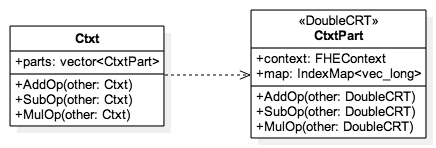
\includegraphics[width=0.65\textwidth]{CtxtTypeHierarchy.png}
\caption{HElib Type Hierarchy}
\label{fig:CtxtTypeHierarchy}
\end{figure}
Before addressing the changes present in GPUHElib, it is necessary to understand the current serial implementation of HElib. Let $\ast$ be the operation being perform (here $\ast$ could stand for any of the operations, all of them are handled similarly) and $A$ and $B$ be the ciphertexts being operated on. The execution of the operation $ A = A\ \ast\  B$ requires a few steps. $A$ and $B$ are stored as \verb|Ctxt| objects in HElib. Figure \ref{fig:CtxtTypeHierarchy} shows the type hierarchy for a \verb|Ctxt| object. \verb|Ctxt| objects have one important variable, \verb|parts|, a vector containing multiple \verb|CtxtPart|s. These parts constitute the ciphertext. The operations supported by \verb|Ctxt| are the addition, subtraction, and multiplication of two \verb|Ctxt| objects. Each of these operations use \verb|parts| during the execution of the operation, thus the operations in \verb|CtxtPart| are called.

\verb|CtxtPart| is an extension of the class \verb|DoubleCRT|, which is where the operations are implemented. Below is code for the operations.

\begin{lstlisting}[language=C++,caption={Add, Sub and Mul operations of two DoubleCRT objects}]
...
const IndexSet& s = map.getIndexSet();
long phim = context.zMStar.getPhiM();

for (long i = s.first(); i <= s.last(); i = s.next(i)) {
    long pi = context.ithPrime(i);
    vec_long& row = map[i];
    const vec_long& other_row = (*other_map)[i];

    for (long j = 0; j < phim; j++) {
      row[j] = fun.apply(row[j], other_row[j], pi);
    }
}
...
\end{lstlisting}

As seen in the code above, the index set is iterated over. For each index, the ith prime is extracted along with the ith row from the maps. Even though the map is accessed like an array, it is an unordered map, with the array access syntax for convenience. These rows are then iterated over, applying the operation to each element. This is where the SIMD design is occurring. A double \verb|for| loop to add, subtract or multiply two vectors together. This is where the GPU implementation can occur

\section{Memory Mapping} \label{sec:MemoryMapping}
In order for the GPU to execute a kernel, it must have the data in a 1D vector. This requires that the data be mapped from its current storage model into a 1D vector.

\subsection{HElib Data Storage and Mapping for GPU Implementation}

\begin{figure}[htp]
\centering
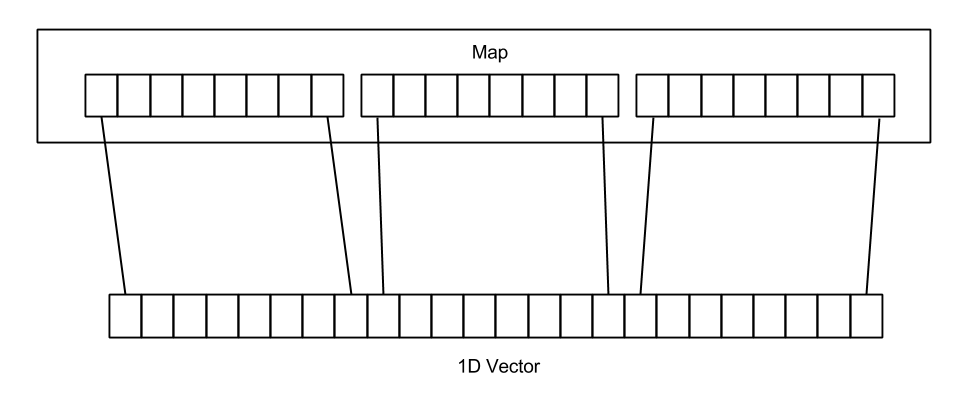
\includegraphics[width=0.65\textwidth]{HElibDataStorage.png}
\caption{HElib Data Storage (Blue area is on CPU, Green area is on GPU)}
\label{fig:HElibDataStorage}
\end{figure}

Currently the data is stored as shown in Figure \ref{fig:HElibDataStorage}. The \verb|map| contains vectors or rows, each of these rows are arrays of 64-bit integers. This structure is a non-contiguous 1D vector that needs to be mapped to a contiguous 1D vector. Thus the rows must be copied into a new vector, which the GPU will then operate on. Each successive row is concatenated to the preceding rows, thus creating a 1D vector.

\begin{figure}[htp]
\centering
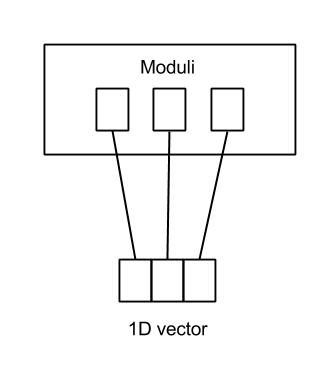
\includegraphics[width=0.3\textwidth]{HElibModuliStorage.png}
\caption{HElib Moduli Storage (Blue area is on CPU, Green area is on GPU)}
\label{fig:HElibModuliStorage}
\end{figure}

Similarly the moduli are being stored as individual elements. In order to be used during execution on the GPU, they must also be mapped to a 1D vector. Figure \ref{fig:HElibModuliStorage} shows the current storage model for the moduli. Each successive modulus is concatenated to the preceding moduli, thus creating a 1D vector.

\section{Overflow Considerations} \label{sec:OverflowConsiderations}
Arithmetic overflow occurs when the result of an arithmetic operation is greater than the magnitude of the storage location that is being used to store the value. For example, using 4-bit unsigned integers, the largest possible value that can be stored is $2^{4} - 1 = 15$. Thus when adding $12 + 14 = 26$, an overflow error will occur, because $26$ requires 5 bits to store. 

The type of the data being operated on in HElib is 64-bit signed integers. Meaning they can take values from $-(2^{63})$ to $2^{63} - 1$. However these values will never be negative, thus the actual range of these values is $0$ to $2^{63} - 1$. The largest modulus could be the largest possible value, $2^{63} - 1$ and the largest value being operated on could be $2^{63} - 2$. The reason that the largest value being operated on is one less than the largest value, $2^{63} - 1$, is because the value has to be smaller than the modulus, thus $(2^{63} - 1) - 1 = 2^{63} - 2$. In CUDA, the language used on NVIDIA GPUs, and the language this implementation is written in, the largest variable type has a length of 64 bits. The type that can contain the largest value is \verb|uint64_t|. This type takes values from 0 to $2^{64} - 1$.

Six operations were designed, as they are the most commonly used operations. Addition, subtraction, and multiplication of a \verb|DoubleCRT| with another \verb|DoubleCRT| and addition, subtraction, and multiplication of a \verb|DoubleCRT| with a constant number. Further considerations for overflow prevention for each operation is discussed in the below sections.

\subsection{Addition Overflow Considerations}
When considering the overflow prevention for addition, it is necessary to compute what the largest value could possibly be. As noted above, the largest a value could be is $2^{63} - 2$ and the largest modulus is $2^{63} - 1$. Performing the addition operation on the possible values, 
\begin{equation} \label{eq:add}
(2^{63} - 2) + (2^{63} - 2) = 2^{64} - 4
\end{equation}
shows that the number $2^{64} - 4$ needs to be computed, before the modulus operation takes place. This number is outside the range for signed 64-bit integers, but not for unsigned 64-bit integers. Thus the original numbers must be cast to unsigned 64-bit integers (which could cause problems if any of the numbers were negative, but since the values are always positive, there is no problem). After the addition operation takes place, the modulus operation brings the result back down the the range of signed integers, because the modulus is in the range of signed integers. The result is then finally cast back to a signed integer, and the operation is complete. The kernels for both addition operations, between two \verb|DoubleCRT| objects and between a \verb|DoubleCRT| object and a constant are in Appendix 
\ref{sec:KernelAddition}.

\subsection{Subtraction Overflow Considerations}
Similar to addition, it is necessary to compute the worst case scenario when considering overflow prevention. Again the largest a value could be is $2^{63} - 2$ and the largest modulus is $2^{63} - 1$. There are two scenarios to consider for subtraction: the first number being $2^{63} - 2$ and the second number being 0 and the first number being 0 and the second number being $2^{63} - 2$. Performing the subtraction operation and modulus calculation for both scenarios,
\begin{equation} \label{eq:sub1}
(2^{63} - 2) - 0 = 2^{63} - 2
\end{equation}
\begin{equation} \label{eq:sub2}
0 - (2^{63} - 2) = -(2^{63} - 2)
\end{equation}
shows that all the computations can be completed using signed integers, because all numbers in the above equations are within the range of signed integers. Thus there does not need to be any steps taken to prevent overflow for this design. 

With this design, to ensure that the resultant value is greater than 0, a check is made after the subtraction operation takes place, to determine if the result is less than 0. If so, the modulus is then added to the value, which will result in the value being larger than 0. This check will cause a branch to occur in the GPU, which could slow down run-time. Alternatively, instead of performing a check to determine if the result is less than 0, the modulus can be added to the first value, then the second is subtracted, shown in the below equation, which is a different approach to the subtraction operation. Equation \ref{eq:sub2} is redefined below, with this procedure applied. 
\begin{equation}
(0 + (2^{63} - 1)) - (2^{63} - 2) = (2^{63} - 1) - (2^{63} - 2) = 1
\end{equation}
Now when the modulus operation occurs, the correct result is found, however none of the values throughout the calculation were ever negative. Thus there is no need to perform a check, avoiding the branch, and possible slow down of the run-time. This method however does result in an overflow issue, because the modulus is being added to the first value. Below is this approach applied to Equation \ref{eq:sub1}.
\begin{equation}
((2^{63} - 2) + (2^{63} - 1)) - 0 = (2^{64} - 3) - 0 = (2^{64} - 3)
\end{equation}
This equation generates the value $2^{64} - 3$, which is too large for the signed integer range. Thus a similar procedure to that of addition is performed to ensure overflow prevention. The original numbers are cast to unsigned 64-bit integers. The operation detailed above takes place, before the modulus operation brings the result back down to the signed integer range. The result is then cast back to a signed integer, and completes the operation. The kernels for both subtraction operations, between two \verb|DoubleCRT| objects and between a \verb|DoubleCRT| object and a constant are in Appendix \ref{sec:KernelSubtraction}.

\subsection{Multiplication Overflow Considerations}
Multiplication presents much more problems compared to addition and subtraction. Again the largest value possible is $2^{63} - 2$, with the largest modulus being $2^{63} - 1$. Performing the multiplication operation on these values, 
\begin{equation} \label{eq:mul}
(2^{63} - 2) * (2^{63} - 2) = 2^{126} - 2^{65} + 4
\end{equation}
shows that very large numbers must be generated when performing the multiplication operation. Where for addition and subtraction the result could fit in a possible data type (unsigned 64-bit integer), these values will not fit in any data type available in CUDA. Therefore an algorithm must be used, which will break up the original numbers into smaller pieces. These pieces will then be used during intermediary steps to generate other values, that when combined back together will result in the correct answer, without ever generating a value that cannot fit in the GPU. The algorithm that is used is Karatsuba's algorithm. 

\subsubsection{Karatsuba's Algorithm}
\begin{equation} \label{eq:Karatsubas}
\begin{split}
x &= x_1 B^m + x_0\\
y &= y_1 B^m + y_0 \cr\\
z_2 &= x_1 y_1\\
z_1 &= x_1 y_0 + x_0 y_1\\
z_0 &= x_0 y_0 \cr\\
xy & = (x_1 B^m + x_0)(y_1 B^m + y_0)\\
 & = z_2 B^{2m} + z_1 B^{m} + z_0
\end{split}
\end{equation}

Equation \ref{eq:Karatsubas} shows Karatsuba's algorithm in general. The values being multiplied are $x$ and $y$. They are broken into pieces $x_1$, $x_0$ and $y_1$, $y_0$ respectively. These pieces are then used to create $z_2$, $z_1$, and $z_0$, which are finally combined with the base number, $B^m$, to generate the original result. For this case, $B=2$ and $m=32$. These values will ensure that operations performed throughout the execution of this algorithm never become greater than the maximum 64-bit unsigned integer value. Each of these will be examined more in-depth to see this.

When $x = 2^{63} - 2$, the variables $x_1$ and $x_0$ have values $x_1 = 2^{31} - 1$ and $x_0 = 2^{32} - 2$. The exact same values are assigned to $y_1$ and $y_0$ since $y = x = 2^{63} - 2$. 

Computing $z_2$,
\begin{equation}
\begin{split}
z_2 & = x_1 y_1\\
 & = (2^{31} - 1) (2^{31} - 1)\\
 & = 2^{62} - 2^{32} + 1
\end{split}
\end{equation}
shows that $z_2$ can fit inside a signed 64-bit integers, since the largest possible value is less than $2^{63} - 1$ (the largest value possible for signed 64-bit integers). 

Computing $z_1$,
\begin{equation}
\begin{split}
z_1 & = x_1 y_0 + x_0 y_1\\
 & = 2[(2^{31} - 1) (2^{32} - 2)]\\
 & = 2[2^{63} - 2^{33} + 2]\\
 & = 2^{64} - 2^{34} + 4
\end{split}
\end{equation}
shows that the intermediate pieces can be computed using signed 64-bit integers, however the addition operation causes the result to be in the range of unsigned 64-bit integers. Thus this calculation requires casting the pieces to unsigned 64-bit integers, carrying out the operation to calculate $z_1$, then performing the modulus operation to bring $z_1$ back down to the signed 64-bit integer space.

Computing $z_0$,
\begin{equation}
\begin{split}
z_0 & = x_0 y_0\\
 & = (2^{32} - 2) (2^{32} - 2)\\
 & = 2^{64} - 2^{34} - 4
\end{split}
\end{equation}
shows that $z_0$ must be calculated using unsigned 64-bit integers, since the result is to large for signed 64-bit integers. Thus this calculation also requires casting the pieces to unsigned 64-bit integers, performing the multiplication, before calculating the modulus to bring the result back into the signed 64-bit integer range.

Now that each of the intermediate pieces have been addressed, the final piece needs consideration. Computing $xy$,
\begin{equation}
\begin{split}
xy & = z_2 B^{2m} + z_1 B^{m} + z_0\\
 & = (2^{62} - 2^{32} + 1) (2^{64})\ +\ (2^{63} - 2^{34} + 5) (2^{32})\ +\ (2^{63} - 2^{34} - 3)
\end{split}
\end{equation}
shows that there will be problems computing $z_2 B^{2m}$ and $z_1 B^{m}$. However these can be dealt with deterministically. By performing a loop, multiplying $z_2$ and $z_1$ by 2, 64 and 32 times respectively, performing the modulus operation after every multiplication, one can obtain the correct value, without exceeding the unsigned 64-bit integer limit. Final modulus operations are applied to each addition, finally resulting in the correct value. This value is cast back to a signed 64-bit integer, and the operation is complete. The kernels for both multiplication operations, between two \verb|DoubleCRT| objects and between a \verb|DoubleCRT| object and a constant are in Appendix \ref{sec:KernelMultiplication}.

\section{Pipelining} \label{sec:Pipelining}
\begin{figure}[htp]
\centering
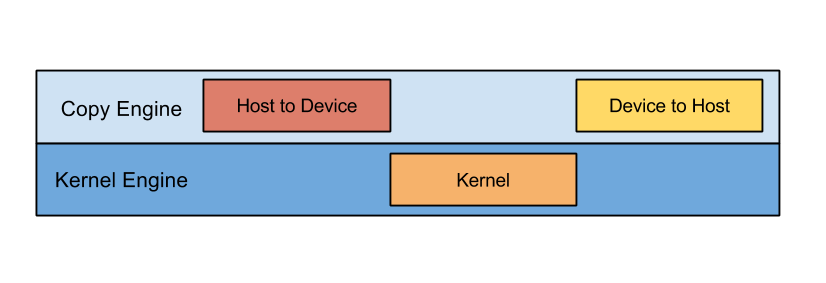
\includegraphics[width=0.65\textwidth]{GPUSerial.png}
\caption{Serial GPU Execution}
\label{fig:GPUSerial}
\end{figure}
As mentioned at the beginning of the chapter, there are three phases when performing operations on a GPU. First the data is copied from the host to the device, then the kernel is executed, and finally the data is copied back from the device to the host. The copy operations are handled by the copy engine, a processor that specifically deals with copying data back and forth from the host and device. Kernels are executed by the kernel engine. This operation is serial, meaning that all the data is copied from the host to device, before the kernel is executed. And the memory is not copied back, until all of the kernels have finished executing. This is illustrated in Figure \ref{fig:GPUSerial}. CUDA allows for these operations to be parallelized, using streams.

\subsection{CUDA Streams}
\begin{figure}[htp]
\centering
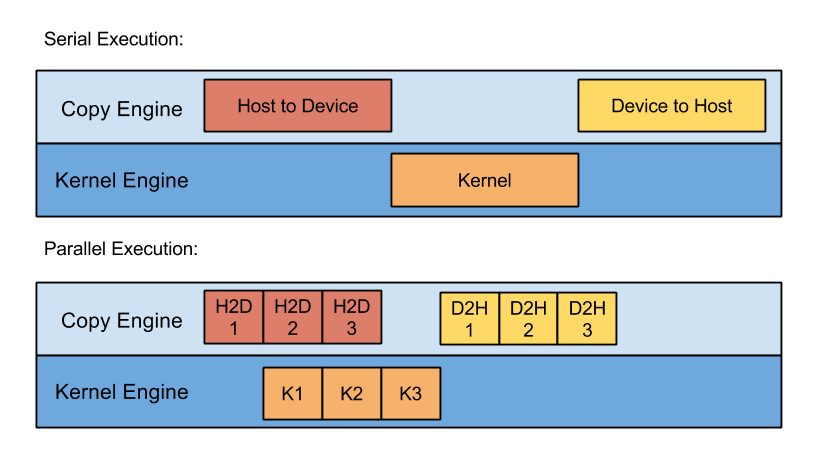
\includegraphics[width=0.65\textwidth]{GPUConcurrent.png}
\caption{Concurrent GPU Execution with 3 Streams}
\label{fig:GPUConcurrent}
\end{figure}
CUDA streams are a sequence of operations that execute in order on a GPU. Operations in different streams can execute concurrently, and be interleaved. Figure \ref{fig:GPUConcurrent}, shows this process applied to the same operations shown in Figure \ref{fig:GPUSerial}. One can see that this allows for speedup, because the copy to/from host to device can be executed, while the kernels are being executed. Streams are useful for parallelizing the computation, however the order in which the operations are dispatched also plays a role.

\subsection{Overlapping Kernel Execution}
There are two ways of dispatching GPU operations: all at once, or by batching similar operations together.

\subsubsection{All At Once Method}
The first approach launches all the operations at once, shown in the code below.
\begin{lstlisting}[language=C++,caption={Operations launched all at once}]
for (int i = 0; i < nStreams; i++) {
    int offset = i * streamSize;
    cudaMemcpyAsync(&d_a[offset], &a[offset], streamBytes, 
                    cudaMemcpyHostToDevice, stream[i]);
    kernel<<<streamSize/blockSize, blockSize, 
                0, stream[i]>>>(d_a, offset);
    cudaMemcpyAsync(&a[offset], &d_a[offset], streamBytes, 
                    cudaMemcpyDeviceToHost, stream[i]);
}
\end{lstlisting}
So all three phases are launched successively on the same stream, before the next stream's operations are launched. 
\subsubsection{Batching Method}
The second approach is to launch similar operations together, instead of all at once. This is show in the code below.
\begin{lstlisting}[language=C++,caption={Operations batched}]
for (int i = 0; i < nStreams; ++i) {
  int offset = i * streamSize;
  cudaMemcpyAsync(&d_a[offset], &a[offset], streamBytes, 
                    cudaMemcpyHostToDevice, stream[i]);
}
for (int i = 0; i < nStreams; ++i) {
  int offset = i * streamSize;
  kernel<<<streamSize/blockSize, blockSize, 
            0, stream[i]>>>(d_a, offset);
}
for (int i = 0; i < nStreams; ++i) {
  int offset = i * streamSize;
  cudaMemcpyAsync(&a[offset], &d_a[offset], streamBytes, 
                    cudaMemcpyDeviceToHost, stream[i]);
}
\end{lstlisting}
In this second approach, all the copy from host to device operations are launched on their respective streams, then the kernels are executed, and finally the device to host copies are dispatched.

Both of these methods will produce the same result, as they are executing the same commands. However depending on the hardware being used, one method might achieve a better speedup over the other.

\subsection{2-Way Pipelining}
\begin{figure}[htp]
\centering
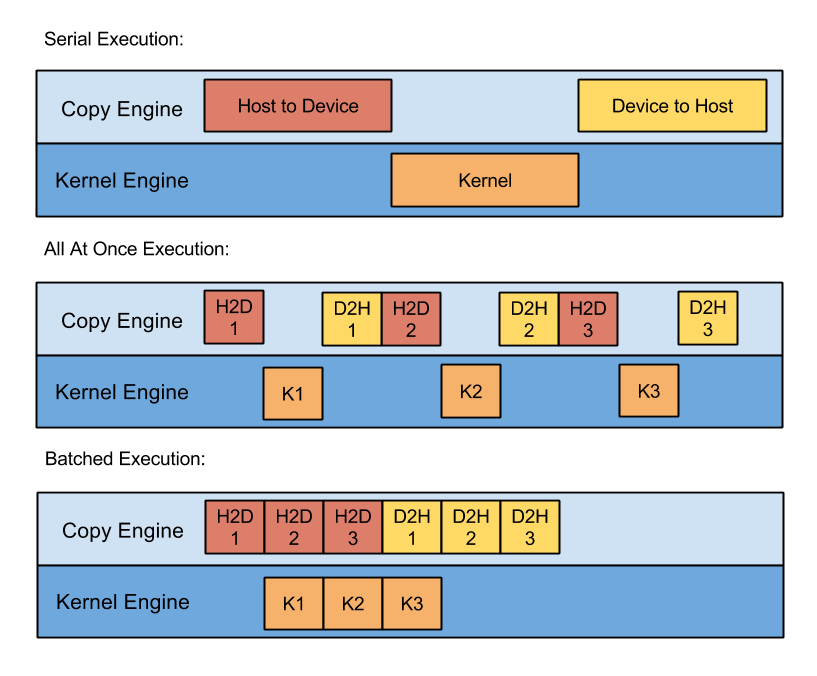
\includegraphics[width=0.65\textwidth]{GPU2Way.png}
\caption{GPU 2-Way Pipelining}
\label{fig:GPU2Way}
\end{figure}
Older GPU hardware only has a single copy engine and a single kernel execution engine. Figure \ref{fig:GPU2Way} shows both methods of kernel execution compared to serial execution. As one can see, both provide a speed up, however the batching method provides a greater speedup over the all at once method. This is because the all at once method launched the second copy from host to device after the first copy from device to host. Because there is only one copy engine, and the engine executes operations in the order they were launched, the copy engine must execute the copy from device to host, before the next host to device copy can occur. Using the second method though, the copies from host to device are all launched before the copies from device to host, so they call all execute one after the other. This allows for the most efficient pipelining, and the greatest speedup on hardware that only has one of each engine.
\subsection{3-Way Pipelining}
\begin{figure}[htp]
\centering
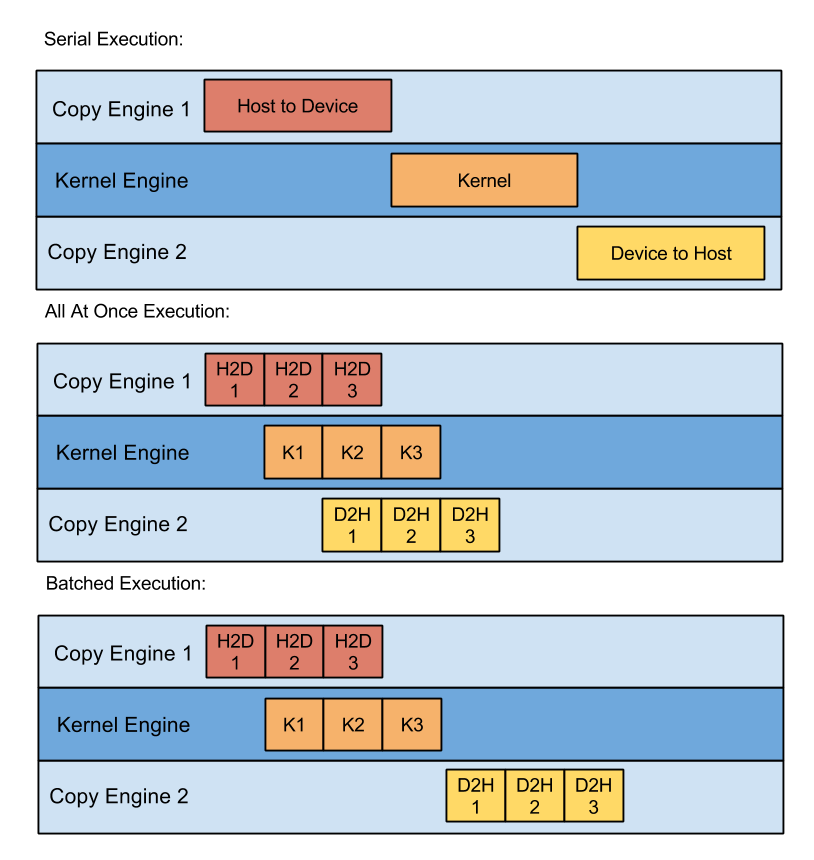
\includegraphics[width=0.65\textwidth]{GPU3Way.png}
\caption{GPU 3-Way Pipelining}
\label{fig:GPU3Way}
\end{figure}
Newer GPU hardware have both a copy from host to device and copy from device to host engines, as well as the kernel engine. The two methods under this new hardware configuration are shown in Figure \ref{fig:GPU3Way}. Here one can see that again both methods provide an overall speedup, however for this case, the all at once method achieves the greatest speedup. Even though the first device to host copy was issued before the second host to device copy in the all at once method, the second host to device copy can be executed earlier than it because of the two copy engines. This is what is allowing the all at once execution method to be faster than the batching method. The batching method is suffering from a design choice in the scheduler of the GPU. The GPU tries to execute the kernels concurrently, and in doing so, delays a signal telling the device to host to starting copying until all the kernels have finished execution.
\chapter{DistributedHElib Design} \label{chap:DistributedHElibDesign}
The second attempt at speeding up the run-time of HElib utilizes a cluster of compute nodes to parallelize operations. A cluster of nodes is a connected group of machines that communicate with each other to achieve a common task. By delegating separate work to each machine, work can be split between many machines, instead of having a single machine handle the entire work load. By doing this, run-times can increase, especially if each node is working on completing an independent task, which helps complete an overall global task. As discussed in the beginning of Chapter \ref{chap:GPUHElibDesign}, HElib utilizes a SIMD design, meaning that a single instruction or operation is performed over many pieces of independent data. With a distributed design then, the hope is to split the data up, send it to compute nodes, have those nodes perform the operations, and send the results back. Having each node work simultaneously on separate pieces of the data, can allow for a speedup in run-time compared to only having a single machine work on all the data.

For this design, a master-slave architecture was chosen. This means that there will be one node, the dispatcher node, which controls the other nodes, the compute nodes. The dispatcher node will be running HElib and when needed, will assign work to the compute nodes. There are a few phases when executing operations in a distributed computing environment.

First the cluster must be setup, and nodes must be designated as compute or dispatcher nodes. Then the dispatcher node must assign work to the compute nodes. As part of assigning work, the dispatcher node must partition the data, and send the pieces to the respective compute nodes. The compute nodes must then perform the operations, and send the data back. Finally the dispatcher node collects all the results and stores them, before returning to regular execution. The cluster setup and work assignment phases are discussed in Section \ref{sec:NodeClusterSetup}. The partitioning of the data is discussed in Section \ref{sec:DistributedMemoryMapping}. Finally the methods by which the data is transmitted between nodes is discussed in Section \ref{sec:Concurrency}.
 
\section{Node Cluster Setup} \label{sec:NodeClusterSetup}
Upon startup of a cluster of nodes, each must be assigned a job. For this design a master-slave architecture is used. This means that one node must be designated the master node, which will be the dispatcher node, and the others are designated slave nodes, or compute nodes. The dispatcher node is the node responsible for running the serial portion of HElib, and distributing the data to the worker nodes when a distributed part of computation is reached. The compute nodes just wait for instructions from the dispatcher node, and act accordingly when given tasks.

When starting a cluster with OpenMPI, the distributed computing communication interface, each node is assigned a number, starting at $0$ through $num\_nodes - 1$. Node $0$ becomes the dispatcher node, and the others are compute nodes. The dispatcher node then returns to normal program execution, while the compute nodes wait for messages from the dispatcher node. 

When the dispatcher node reaches a point of execution that is meant to be distributed, it partitions the data (discussed in Section \ref{sec:DistributedMemoryMapping}) and assigns each compute node a piece of the data to operate on. The manner in which the dispatcher node chooses what compute node will operate on what piece of data is examined next.

\subsection{Work Assignment}
After the data has been partitioned, it must be assigned to a compute node to be operated on. The scheme used to choose the next compute node for a piece of data is round-robin scheduling. This scheme allows for an even or almost even distribution of the data across all the compute nodes. Having an even or almost even distribution means the lowest run-times and the best efficiency. There are two cases to consider when determining if a distribution scheme is efficient: when there are more compute nodes than data pieces, and when there are fewer compute nodes than data pieces.

\begin{figure}[htp]
\centering
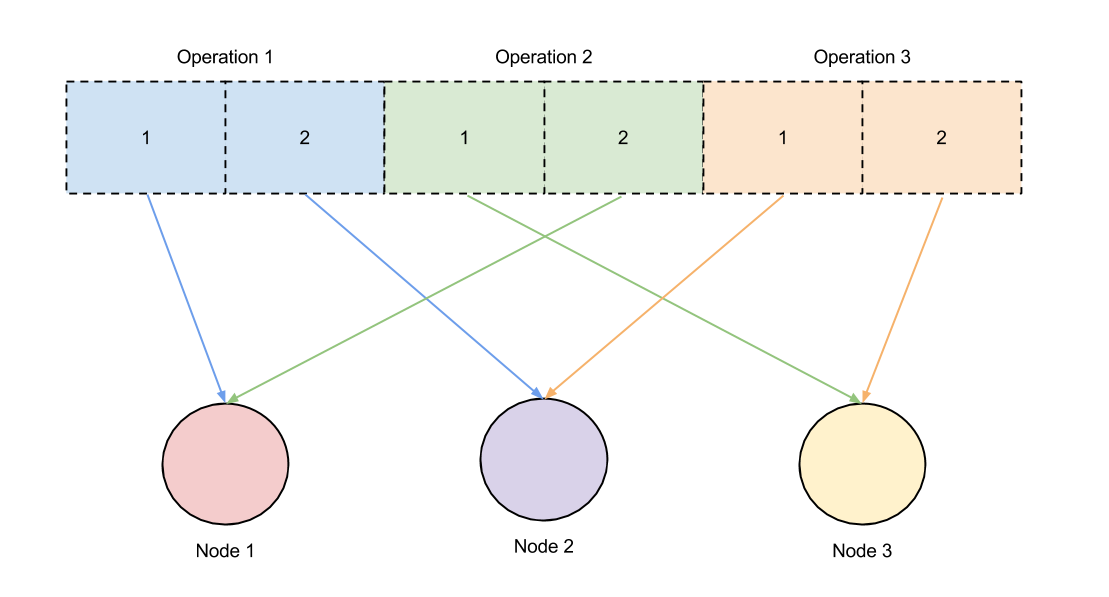
\includegraphics[width=0.95\textwidth]{RollingRoundRobinExampleMore.png}
\caption{Rolling Round Robin Example with More Nodes than Data Pieces}
\label{fig:RollingRoundRobinExampleMore}
\end{figure}
For the first case, with the round-robin scheduling, this just means that some nodes will not be working, while others are. For this design a rolling round-robin design is used. This means that for any operations, the next node to be assigned work will always be the node which was assigned work the longest time ago. This node has the highest probability of being free and ready to receive more work, compared to all the others. Figure \ref{fig:RollingRoundRobinExampleMore} shows an example of rolling round-robin scheduling applied to this case.

\begin{figure}[htp]
\centering
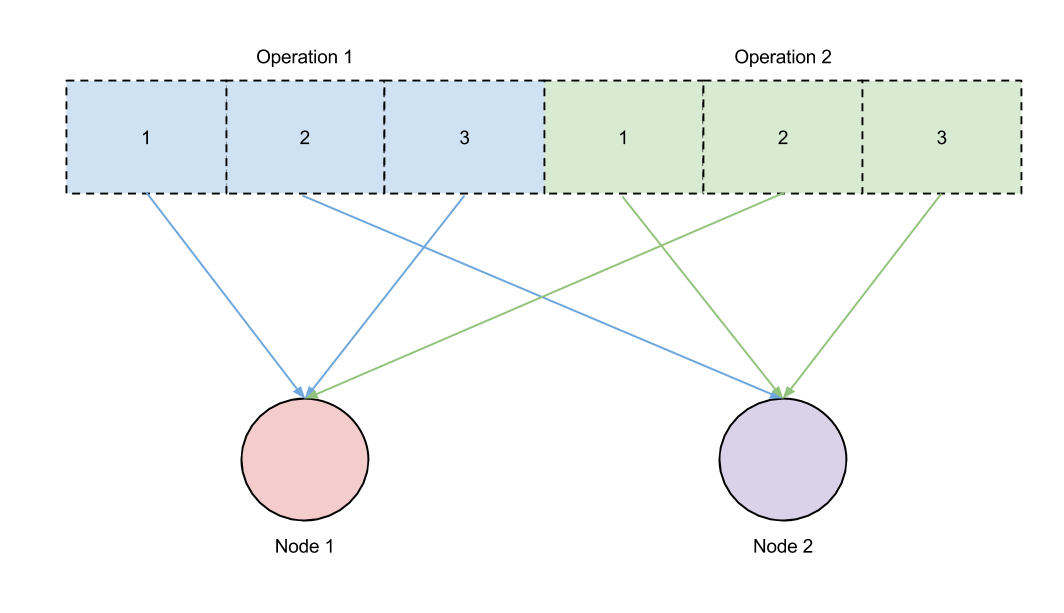
\includegraphics[width=0.95\textwidth]{RollingRoundRobinExampleLess.png}
\caption{Rolling Round Robin Example with Less Nodes than Data Pieces}
\label{fig:RollingRoundRobinExampleLess}
\end{figure}
For the second case, with the round-robin scheduling, this just means that some nodes will have multiple pieces of data to operate on. By using the round-robin scheduling though, the amount of work done by each compute node should be about equal, and thus evenly spread over the compute nodes. If work was unequally proportioned to a single compute node, compared to others, then the dispatcher node might have to wait longer for the results, before continuing normal execution. This way the greatest run-time and efficiency is achieved. Figure \ref{fig:RollingRoundRobinExampleLess} shows an example of rolling round-robin scheduling applied to this case.

\section{Memory Mapping} \label{sec:DistributedMemoryMapping}
In order for the compute nodes to execute, they must have a portion of the data to work on. This requires the dispatcher node to partition the data from its current storage model into pieces, before they are sent to the compute nodes to be worked on.

\subsection{Mapping from Dispatcher Node to Compute Nodes}
\begin{figure}[htp]
\centering
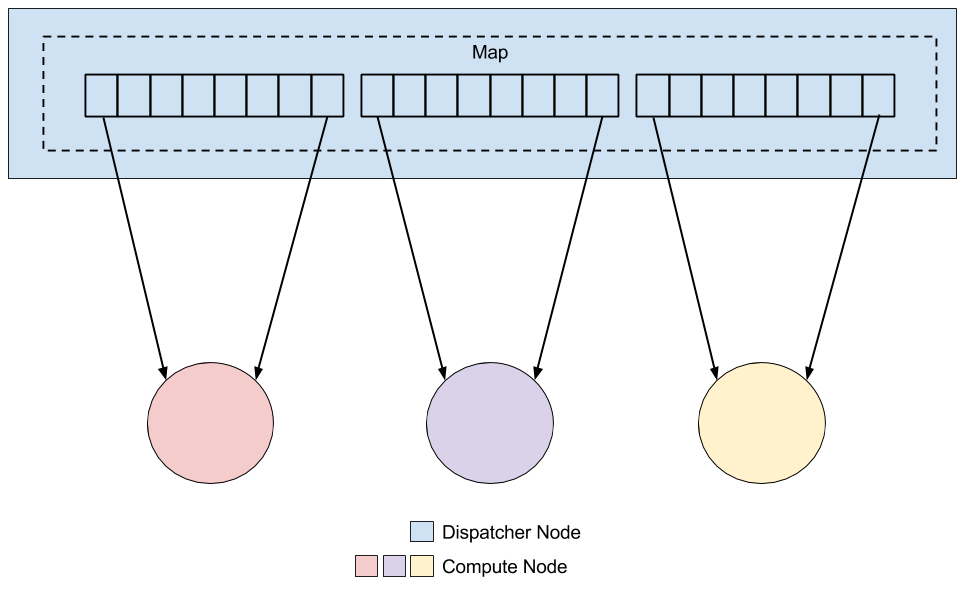
\includegraphics[width=0.65\textwidth]{MappingDispatchertoComputeData.png}
\caption{Data Mapping from Dispatcher to Compute Nodes}
\label{fig:MappingDispatcherToComputeData}
\end{figure}
Currently the data is stored as shown in Figure \ref{fig:MappingDispatcherToComputeData}. The \verb|map| contains vectors or rows, each of these rows are arrays of 64-bit integers. The rows present a great partitioning point. Splitting the data up by these rows, and sending individual rows to each compute node to be operated on, is the logical splitting point because there will always be about the same number of rows during execution, however the size of the rows might change drastically. Also, splitting rows up would cause more communication between the nodes, which could slow down run-times. 

\begin{figure}[htp]
\centering
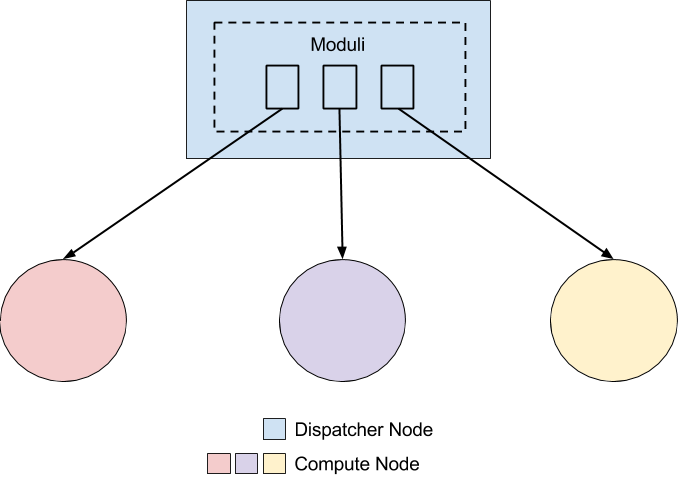
\includegraphics[width=0.65\textwidth]{MappingDispatchertoComputeModuli.png}
\caption{Moduli Mapping from Dispatcher to Compute Nodes}
\label{fig:MappingDispatcherToComputeModuli}
\end{figure}
Similarly the moduli are being stored as individual elements. Because each moduli is assigned to each row, and the rows are being assigned to a single compute node, each moduli must only be sent to the specific compute node that the row it corresponds to is on. Figure \ref{fig:MappingDispatcherToComputeModuli} shows the mapping process. Each modulus is only sent to the compute node that its corresponding row is sent to.

\subsection{Compute Node Vector Management}
Naively creating and freeing buffers on the compute nodes that will receive the data from the dispatcher node slows down run-times. By creating a few buffers, and maintaining them throughout the programs lifetime, the most efficient memory usage is achieved, along with the greatest speedup.

Two buffers are created and maintained throughout the lifetime of the program. Both buffers are of size $size\_of\_row$. These are the buffers that the rows will be copied into on the compute nodes. The size, $size\_of\_row$, rarely changes, thus there will be little memory reallocation occurring. Also, reallocation will only occur when the buffer is too small, not when it is larger than needed. So the buffer will only ever grow, not shrink, thus cutting down on the occurrences of reallocation needing to be performed. The function that handles initializing and reallocation of these buffers is found in Appendix \ref{sec:ComputeNodeBufferManagement}.

\section{Concurrency} \label{sec:Concurrency}
Concurrency for a distributed system means that each node is executing operations simultaneously. To achieve concurrency in this system, the dispatcher node must be able to assign work, and not have to wait for a response, before assigning more work and the compute nodes must be able to perform computations at the same time. For all of these operations to happened concurrently, the communication between the nodes must be non-blocking.

\subsection{Non-Blocking Send and Receive with OpenMPI}
Blocking send and receive functions require the data to be completely sent or received before continuing execution. This means that if a node were to call \verb|receive|, it would wait until it received data, before continuing execution. This can both be beneficial and detrimental, depending on the needs of the design. Non-blocking send and receive functions however schedule requests, and then continue execution. These requests will later be filled, but execution can continue, even if they have not yet been filled. So a request can be generated, and even if the data has not finished sending or been completely received, execution can continue. This request can then be tested, and once the data has been sent or received, the request will be filled. Both methods have there uses, discussed next.

\subsubsection{Send and Receive on Compute Nodes}
For the compute nodes, blocking send and receive functions are used, because it is necessary for the buffer holding the result of the operation to be sent back to the dispatcher node, before the next operation occurs. If the next operation occurred before the dispatcher node received the data, the buffer could be cleared or overwritten, and the data sent back would be incorrect.

\subsubsection{Send and Receive on Dispatcher Node}
For the dispatcher node, non-blocking send and receive functions are used. This allows the dispatcher node to continue assigning work, even if the compute nodes have not fully received their assigned work. Also the dispatcher node will use non-blocking receive functions in order to receive data back as quickly as possible. If the dispatcher node used blocking receive functions, then it could be waiting on a node that is taking a long time to perform an operation, and causing other compute nodes to wait that might have already finished computation, and may have pending computation that they could be moving onto. 

Only using non-blocking receive functions could cause problems for the dispatcher node, if for example two operations are performed, and the second requires the results from the first. Without any mechanisms to ensure the result to the first operation is received, before the execution of the second operation, unknown results can be computed. Therefore there is a need for a syncing mechanism.

\subsection{Syncing}
A syncing mechanism will cause the dispatcher node to wait for all pending requests to be completed before continuing execution. In this way, it can be ensured that a single operation is fully completed before moving onto other operations. To keep track of these requests a linked list is used. When a new request is created, through either a call to \verb|send| or \verb|receive|, it is added to the end of the linked list. When the \verb|sync| function is called, each of these is tested to see if they have completed. If a request has been completed, then it is removed from the linked list, if not, the function moves onto the next in the list, and checks it. The function only returns when all the pending requests have been filled, when the linked list is empty. The \verb|sync| function can be found in Appendix \ref{sec:SyncFunction}. A \verb|sync| operation is performed after every operation to ensure that the operation is completed, before moving onto the next operation.
\chapter{Evaluation} \label{chap:Evaluation}
The evaluation of this work has two objectives. First, to make sure that the modified designs still produce correct output. Meaning that the result of an operation when decrypted is the same for both the modified and unmodified versions of the library. Secondly, to profile each design and compare run times of the modified libraries to the unmodified library. These time comparisons will occur at multiple levels to best understand each design, and how they compare to the serial version.

Distributed systems achieve the best efficiency when working on large inputs, not small ones. This is because there is some overhead associated with setting up and distributing work. For GPU designs, this overhead time happens when transferring the data to and from the GPU. For distributed computing designs, the overhead time is also in the memory transfers like the GPU, but instead of transferring to the GPU, the memory transfers are between machines. This overhead costs time, that when working with small inputs, usually takes even longer than the operation to complete. Thus the distributed design causes a run time slow down compared to the serial version for small input sizes. However, when working with large amounts of data, the time saved to complete the operation is so great, that the overhead costs are worth it. This characterization of distributed systems is prevalent for these designs, which will be seen later. For these encryption systems, large input sizes occur when $size\_of\_row$ is large. As discussed in the design chapters, $size\_of\_row$ is the length of the vectors in \verb|map|. To best demonstrate the effect $size\_of\_row$ has on the system, $size\_of\_row$ is steadily increased during the testing, so that its effect on each design can be seen and compared to the original design.

To evaluate these designs a few profiling tools were used, discussed in Section \ref{sec:EvaluationTools}. The test environments used for each design are detailed in Section \ref{sec:TestingEnvironment}. The results for GPUHElib are examined in Section \ref{sec:GPUHElibEvaluationResults}, followed by the results for DistributedHElib in Section \ref{sec:DistributedHElibEvaluationResults}. Finally some conclusions are drawn regrading both of these designs in Section \ref{sec:EvaluationConclusions}

\section{Evaluation Tools} \label{sec:EvaluationTools}
The following tools were used to evaluate the correctness of the modified libraries and record run times at various levels in the library.

\subsection{Test Program}
A test program was created based on testing programs provided with the original unmodified version of HElib. This new test program first sets up the ciphertexts that are used during computation. Two ciphertexts are created, both are the integers, $0$ to $ num\_slots\_in\_plaintext$. 

Three operations are reported on in this document, of the six implemented. They are addition, subtraction, and multiplication of one ciphertext with another ciphertext. The other three operations supported, addition, subtraction, and multiplication of a ciphertext and a number, were not reported, as preliminary tests showed that they displayed similar results to their ciphertext only counterparts. It was decided that for conciseness and to avoid repetition, that they would be left out of this document.

The program requires that the user pass in the $size\_of\_row$ they would like to use, which as discussed above, will be incremented during testing. The test program then performs each operation, checking the decrypted result after each operation to make sure that the results are correct, before moving on. Timing blocks were placed around each operation to record the overall time it took to perform the operation. The timers were printed out after each operation. Lower level timers, discussed below, were reset after each operation, so that the lower level times reported with each operation were only times recorded for that operation.

This test program was compiled twice for both designs, first linking against the unmodified library, and second against the modified library. This produced two executables, that were then run to generate the results described below.

\subsection{HELib Timing Functions}
The standard version of HElib provides fine grained timing functions that can be placed anywhere throughout the library. To utilized these functions is simple. First a timer is created. Upon the creation of the timer, it is started. A call to \verb|stop| is made in code when the timer should stop. A timer can be started and stopped multiple times, and the average time will be recorded. The timers are stored in a map, and can be reset if needed. This setup allows for fine grained measurement of functions and detailed profiling of run times. 

Each design, serial HElib, GPUHElib, and DistributedHElib required the timers be placed at some similar places, for comparison purposes, and some distinct places, in order to assess the efficiency of each unique design.

\subsubsection{Serial HElib Timer Placement}
There were two levels at which timers were placed, with each successive level more fine grained. The first level was in the test program, described above. This is the circuit level. The other timer was placed at the function level, inside the function that performed the operations in \verb|DoubleCRT|. This function was where the double \verb|for| loop was located that both of the distributed designs are trying to improve upon.

\subsubsection{GPUHElib Timer Placement}
For GPUHElib, there are three levels at which timers were placed. As described above, the first timer was placed at the circuit level in the test program. This records the time that the entire operation took. The second level of timing was the function level. At this level a timer was placed in the function that is performing the operations in \verb|DoubleCRT|. These first two timer levels allow for comparison against the serial version, as the serial version also has timers placed at these levels. The third and lowest level is the phase level. Four timers are placed at this level to record the setup (vector and stream creation), phase one (host to device memory transfer), phase two (GPU computation), and phase three (device to host memory transfer) times. The timers at this level allow for the times gathered at level two to be broken down even further, and allow each phase of level two to be examined closer.

\subsubsection{DistributedHElib Timer Placement}
For DistributedHElib, there are three levels at which timers were placed. The first at the circuit level in the test program. The second at the function level, in \verb|DoubleCRT|, where the operation is being performed. These first two timer levels are necessary for the comparison against the serial version, as the serial version also has timers at these two levels. The third consists of two timers: the distribute (where the job assignment and data partitioning happens) and the wait (where the sync function is called, and the dispatcher node is waiting for the compute nodes to finish and send back their results). This third level allows for a breakdown of the function level for further analysis. 

\section{Testing Environment} \label{sec:TestingEnvironment}
Both systems required unique testing environments that had the capabilities needed for each design. Both variants used machines with 64-bit Intel Core 2 Duo CPUs running at 3.0 Ghz with about 4 Gb of DDR2, 800 Mhz RAM.

\subsection{GPU Testing Environment}
GPUHElib was tested on a machine with a NVIDIA Quadro NVS 290 GPU, which has 256 MB of RAM. Also this particular GPU only has one copy engine. Thus the tests reported here are using the 2-Way Pipelining design discussed in Section \ref{sec:Pipelining}. CUDA version 6.5 was used.

\subsection{Distributed Computing Testing Environment}
DistributedHElib was tested on a cluster of machines all connected through Ethernet. OpenMPI version 1.8.5 was used. Three cluster configurations were used, one with 4 nodes, one with 8 nodes, and one with 16 nodes.

\section{GPUHElib Evaluation Results} \label{sec:GPUHElibEvaluationResults}
As discussed earlier in this chapter, GPUHElib has three levels of timing information begin recorded. The first, and highest level, is the circuit level, where the high level operation is being computed. The second level is the function level, inside \verb|DoubleCRT| where the \verb|parts| are being operated on. And the lowest level is the phase level, where timing results are recorded for all four phases of the operation. The timing results for each of these levels is discussed in more detail in the following sections.

\subsection{GPUHElib Circuit Level Run Times}
\begin{table}[p]
\centering
\begin{tabular}{ | r | r | r | r | r | r | r | }
 \multicolumn{1}{ r }{} & \multicolumn{6}{ c }{$size\_of\_row$} \\ \cline{2-7}
 \multicolumn{1}{ r |}{} & $1{,}000$ & $10{,}000$ & $100{,}000$ & $200{,}000$ & $300{,}000$ & $400{,}000$ \\ \hline
 Add & 1.400E-05 & 1.080E-04 & 2.545E-03 & 5.396E-03 & 5.354E-03 & 1.053E-02 \\ \hline
 Sub & 1.400E-05 & 1.300E-04 & 2.532E-03 & 5.304E-03 & 5.366E-03 & 1.075E-02 \\ \hline
 Mul & 4.962E-03 & 1.036E-01 & 1.157 & 2.648 & 7.217 & 1.232E+01 \\ \hline
\end{tabular}
\caption{Serial HElib circuit level run times (in seconds)}
\label{tab:GPUserialLevel1Runtimes}
\end{table}

\begin{table}[p]
\centering
\begin{tabular}{ | r | r | r | r | r | r | r | }
 \multicolumn{1}{ r }{} & \multicolumn{6}{ c }{$size\_of\_row$} \\ \cline{2-7}
 \multicolumn{1}{ r |}{} & $1{,}000$ & $10{,}000$ & $100{,}000$ & $200{,}000$ & $300{,}000$ & $400{,}000$ \\ \hline
 Add & 1.050E-03 & 1.675E-03 & 8.972E-03 & 1.646E-02 & 1.671E-02 & 3.704E-02 \\ \hline
 Sub & 1.012E-03 & 1.805E-03 & 9.023E-03 & 1.683E-02 & 1.682E-02 & 3.700E-02 \\ \hline
 Mul & 1.106E-02 & 1.187E-01 & 1.309 & 2.868 & 7.393 & 9.333 \\ \hline
\end{tabular}
\caption{GPUHElib circuit level run times (in seconds)}
\label{tab:GPULevel1Runtimes}
\end{table}

\begin{figure}[p]
\centering

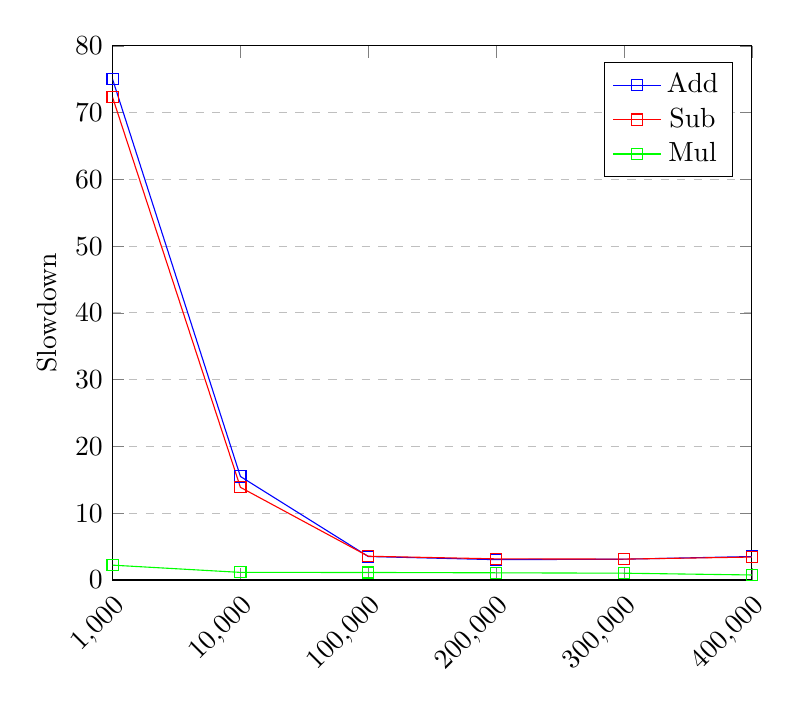
\begin{tikzpicture}
\begin{axis}
[
    ylabel={Slowdown},
    width=.8\textwidth,
    xmin=1, xmax=6,
    ymin=0, ymax=80,
    xtick={1,2,3,4,5,6},
    xticklabels={$1{,}000$, $10{,}000$, $100{,}000$, $200{,}000$, $300{,}000$, $400{,}000$},
    ytick={80,70,60,50,40,30,20,10,0},
    legend pos=north east,
    ymajorgrids=true,
    grid style=dashed,
    x tick label style={rotate=45,anchor=north east},
]

\addplot[color=blue,mark=square]
    coordinates {
    (1,75)(2,15.50925926)(3,3.525343811)(4,3.049481097)(5,3.121404557)(6,3.519144893) };
    
\addplot[color=red,mark=square]
    coordinates {
    (1,72.28571429)(2,13.88461538)(3,3.563586098)(4,3.172511312)(5,3.1339918)(6,3.441354293) };

\addplot[color=green,mark=square]
    coordinates {
    (1,2.229544538)(2,1.146005137)(3,1.131587363)(4,1.083041024)(5,1.024489643)(6,0.757830934) };
    
\legend{Add,Sub,Mul}
 
\end{axis}
\end{tikzpicture}

\caption{Run Time Comparison at Circuit Level}
\label{fig:level1ComparisonSerialGPU}
\end{figure}

Table \ref{tab:GPUserialLevel1Runtimes} and Table \ref{tab:GPULevel1Runtimes} display the run times for serial HElib and GPUHElib tests respectively. Both tests were run with inputs sizes starting at 1,000 and increasing until 400,000. 

Figure \ref{fig:level1ComparisonSerialGPU} visualizes these times as the slowdown of GPUHElib over serial HElib. A value of 1 means that the serial version and the GPU version had the same run time. Above 1 means that the GPU design has a slower run time, and below 1 means that the GPU has a faster run time.

One can see in Figure \ref{fig:level1ComparisonSerialGPU} that for the smaller input sizes, the run times for the GPU are much larger than the serial version for addition and subtraction. They start off taking about 72 times as long to complete compared to the serial version. The multiplication operation also starts off taking longer, however only about 2.2 times as long. The run times for serial HElib and GPUHElib get closer and closer, as the inputs sizes approach 400,000. The addition and subtraction circuit run times minimize at about 3 times as long, for the 300,000 size input. However for the 400,000 size input, the times go in the opposite direction desired, becoming about 3.5 times as long. The multiplication circuit actually has the best results, with the 400,000 test taking about .75 times the serial version. So the multiplication circuit took about 3/4 the time to complete in GPUHElib compared to the serial version. While this result might look good, further analysis of the lower level tests show that this was probably not caused by the usage of the GPU, but by other operations computed during the multiplication operation being faster. The function level run times will be examined next.

\subsection{GPUHElib Function Level Run Times}
\begin{table}[p]
\centering
\begin{tabular}{ | r | r | r | r | r | r | r | }
 \multicolumn{1}{ r }{} & \multicolumn{6}{ c }{$size\_of\_row$} \\ \cline{2-7}
 \multicolumn{1}{ r |}{} & $1{,}000$ & $10{,}000$ & $100{,}000$ & $200{,}000$ & $300{,}000$ & $400{,}000$ \\ \hline
 Add & 5.000E-06 & 4.825E-05 & 1.007E-03 & 2.648E-03 & 2.653E-03 & 5.466E-03 \\ \hline
 Sub & 5.000E-06 & 6.150E-05 & 1.259E-03 & 2.644E-03 & 2.674E-03 & 5.366E-03 \\ \hline
 Mul & 2.900E-05 & 2.830E-04 & 2.879E-03 & 5.863E-03 & 5.856E-03 & 1.176E-02 \\ \hline
\end{tabular}
\caption{Serial HElib function level run times (in seconds)}
\label{tab:GPUserialLevel2Runtimes}
\end{table}

\begin{table}[p]
\centering
\begin{tabular}{ | r | r | r | r | r | r | r | }
 \multicolumn{1}{ r }{} & \multicolumn{6}{ c }{$size\_of\_row$} \\ \cline{2-7}
 \multicolumn{1}{ r |}{} & $1{,}000$ & $10{,}000$ & $100{,}000$ & $200{,}000$ & $300{,}000$ & $400{,}000$ \\ \hline
 Add & 5.210E-04 & 8.298E-04 & 4.392E-03 & 8.257E-03 & 8.346E-03 & 1.864E-02 \\ \hline
 Sub & 5.020E-04 & 8.950E-04 & 4.498E-03 & 8.398E-03 & 8.395E-03 & 1.848E-02 \\ \hline
 Mul & 5.302E-04 & 1.006E-03 & 6.599E-03 & 1.273E-02 & 1.276E-02 & 2.687E-02 \\ \hline
\end{tabular}
\caption{GPUHElib function level run times (in seconds)}
\label{tab:GPULevel2Runtimes}
\end{table}

\begin{figure}[p]
\centering
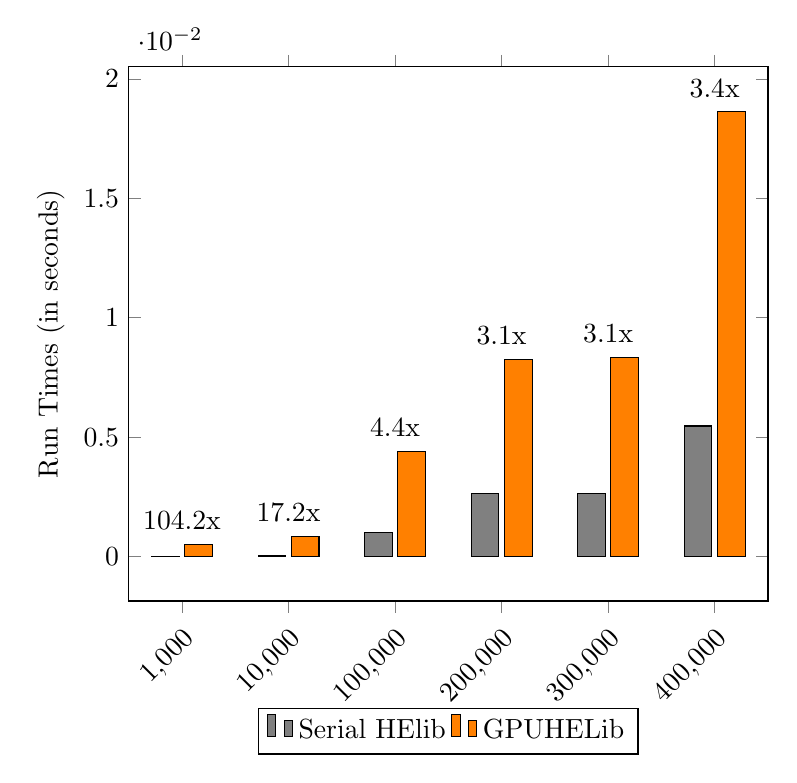
\begin{tikzpicture}

\begin{axis}[
    ybar,
    width=.8\textwidth,
    legend style={at={(0.5,-0.2)},anchor=north,legend columns=-1},
    ylabel=Run Times (in seconds),
    symbolic x coords={$1{,}000$,$10{,}000$,$100{,}000$,$200{,}000$,$300{,}000$,$400{,}000$},
    xtick=data,
    x tick label style={rotate=45,anchor=north east},
]

\addplot[fill=gray]
    coordinates {
    ($1{,}000$,5.000E-06)($10{,}000$,4.825E-05)($100{,}000$,1.007E-03)($200{,}000$,2.648E-03)($300{,}000$,2.653E-03)($400{,}000$,5.466E-03) };
    
\addplot[fill=orange]
    coordinates {
    ($1{,}000$,5.210E-04)($10{,}000$,8.298E-04)($100{,}000$,4.392E-03)($200{,}000$,8.257E-03)($300{,}000$,8.346E-03)($400{,}000$,1.864E-02) };
    
\node at (axis cs:$1{,}000$,1.52E-03) {104.2x};
\node at (axis cs:$10{,}000$,1.83E-03) {17.2x};
\node at (axis cs:$100{,}000$,5.39E-03) {4.4x};
\node at (axis cs:$200{,}000$,9.26E-03) {3.1x};
\node at (axis cs:$300{,}000$,9.35E-03) {3.1x};
\node at (axis cs:$400{,}000$,1.96E-02) {3.4x};
    
\legend{Serial HElib,GPUHELib}
\end{axis}
\end{tikzpicture}

\caption{Add Run Times Comparison at Function Level}
\label{fig:level2ComparisonSerialGPUAddVecs}
\end{figure}

\begin{figure}[p]
\centering
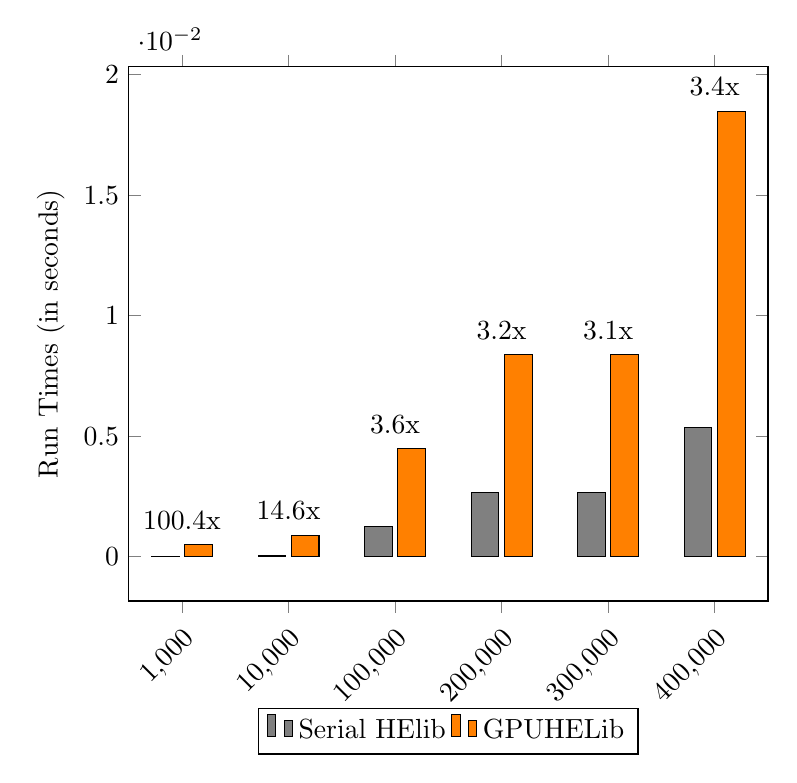
\begin{tikzpicture}

\begin{axis}[
    ybar,
    width=.8\textwidth,
    legend style={at={(0.5,-0.2)},anchor=north,legend columns=-1},
    ylabel=Run Times (in seconds),
    symbolic x coords={$1{,}000$,$10{,}000$,$100{,}000$,$200{,}000$,$300{,}000$,$400{,}000$},
    xtick=data,
    x tick label style={rotate=45,anchor=north east},
]

\addplot[fill=gray]
    coordinates {
    ($1{,}000$,5.000E-06)($10{,}000$,6.150E-05)($100{,}000$,1.259E-03)($200{,}000$,2.644E-03)($300{,}000$,2.674E-03)($400{,}000$,5.366E-03) };
    
\addplot[fill=orange]
    coordinates {
    ($1{,}000$,5.020E-04)($10{,}000$,8.950E-04)($100{,}000$,4.498E-03)($200{,}000$,8.398E-03)($300{,}000$,8.395E-03)($400{,}000$,1.848E-02) };

\node at (axis cs:$1{,}000$,1.50E-03) {100.4x};
\node at (axis cs:$10{,}000$,1.90E-03) {14.6x};
\node at (axis cs:$100{,}000$,5.50E-03) {3.6x};
\node at (axis cs:$200{,}000$,9.40E-03) {3.2x};
\node at (axis cs:$300{,}000$,9.39E-03) {3.1x};
\node at (axis cs:$400{,}000$,1.95E-02) {3.4x};
    
\legend{Serial HElib,GPUHELib}
\end{axis}
\end{tikzpicture}

\caption{Sub Run Times Comparison at Function Level}
\label{fig:level2ComparisonSerialGPUSubVecs}
\end{figure}

\begin{figure}[p]
\centering
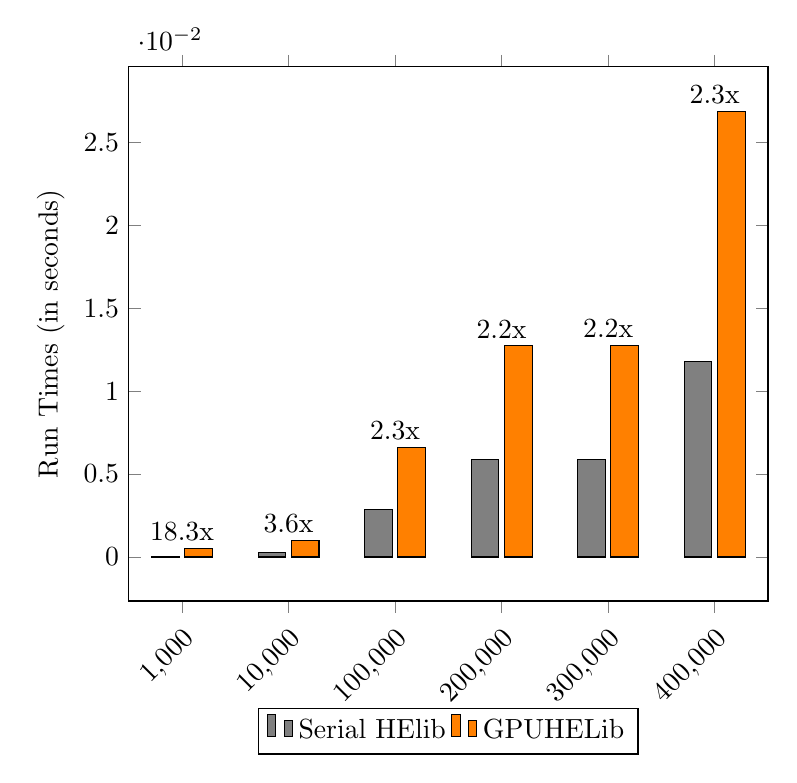
\begin{tikzpicture}

\begin{axis}[
    ybar,
    width=.8\textwidth,
    legend style={at={(0.5,-0.2)},anchor=north,legend columns=-1},
    ylabel=Run Times (in seconds),
    symbolic x coords={$1{,}000$,$10{,}000$,$100{,}000$,$200{,}000$,$300{,}000$,$400{,}000$},
    xtick=data,
    x tick label style={rotate=45,anchor=north east},
]

\addplot[fill=gray]
    coordinates {
    ($1{,}000$,2.900E-05)($10{,}000$,2.830E-04)($100{,}000$,2.879E-03)($200{,}000$,5.863E-03)($300{,}000$,5.856E-03)($400{,}000$,1.176E-02) };
    
\addplot[fill=orange]
    coordinates {
    ($1{,}000$,5.302E-04)($10{,}000$,1.006E-03)($100{,}000$,6.599E-03)($200{,}000$,1.273E-02)($300{,}000$,1.276E-02)($400{,}000$,2.687E-02) };
    					
\node at (axis cs:$1{,}000$,1.53E-03) {18.3x};
\node at (axis cs:$10{,}000$,2.01E-03) {3.6x};
\node at (axis cs:$100{,}000$,7.60E-03) {2.3x};
\node at (axis cs:$200{,}000$,1.37E-02) {2.2x};
\node at (axis cs:$300{,}000$,1.38E-02) {2.2x};
\node at (axis cs:$400{,}000$,2.79E-02) {2.3x};
    
\legend{Serial HElib,GPUHELib}
\end{axis}
\end{tikzpicture}

\caption{Mul Run Times Comparison at Function Level}
\label{fig:level2ComparisonSerialGPUMulVecs}
\end{figure}

Table \ref{tab:GPUserialLevel2Runtimes} and Table \ref{tab:GPULevel2Runtimes} display the run times for the serial HElib and GPUHElib tests respectively. As noted before, both tests were run with input sizes ranging from 1,000 to 400,000.

Figure \ref{fig:level2ComparisonSerialGPUAddVecs}, Figure \ref{fig:level2ComparisonSerialGPUSubVecs}, and Figure \ref{fig:level2ComparisonSerialGPUMulVecs} show the comparisons between the run times for each of the operations at the function level. Also displayed in the figures is the run time slow down of the GPU variant compared to the serial version. So, for example, in Figure \ref{fig:level2ComparisonSerialGPUAddVecs}, the 104.2x above 1,000 means that the GPU variant took 104.2 times longer to complete compared to the serial version.

All these times again reiterate that for the smaller input sizes, the run times for the GPU variant are vastly larger, almost 100x for addition and subtraction, and about 18x for multiplication. As the input sizes increase, the run times get closer and closer, but minimize at about 3.1x for addition and subtraction and at about 2x for multiplication. Again one can see that for the 400,000 input size, the slow downs increase for all the operations compared to the previous input size, 300,000, going from 3.2x to 3.4x and 3.5x respectively and from 2.2x to 2.3x. The results for the multiplication times make it clear that the speedup seen at the circuit level must be caused by other factors than the GPU implementation of multiplication. These times show that multiplication behaves exactly like the other operations in terms of run time patterns. The cause for these slow downs is evident after examining the recorded times at the phase level.

\subsection{GPUHElib Phase Level Run Times}
\begin{table}[p]
\centering
\begin{tabular}{ | r | r | r | r | r | r | r | }
 \multicolumn{1}{ r }{} & \multicolumn{6}{ c }{$size\_of\_row$} \\ \cline{2-7}
 \multicolumn{1}{ r |}{} & $1{,}000$ & $10{,}000$ & $100{,}000$ & $200{,}000$ & $300{,}000$ & $400{,}000$ \\ \hline
 Setup & 2.420E-04 & 2.465E-04 & 2.848E-04 & 3.013E-04 & 3.015E-04 & 3.133E-04 \\ \hline
 Phase 1 & 9.500E-05 & 2.568E-04 & 2.137E-03 & 4.289E-03 & 4.345E-03 & 1.164E-02 \\ \hline
 Phase 2 & 4.425E-05 & 3.350E-05 & 1.283E-04 & 2.423E-04 & 2.420E-04 & 3.728E-04 \\ \hline
 Phase 3 & 1.373E-04 & 2.900E-04 & 1.837E-03 & 3.420E-03 & 3.454E-03 & 6.308E-03 \\ \hline
\end{tabular}
\caption{GPUHElib Add phase level run times (in seconds)}
\label{tab:GPULevel3RuntimesAddVecs}
\end{table}

\begin{figure}[p]
\centering
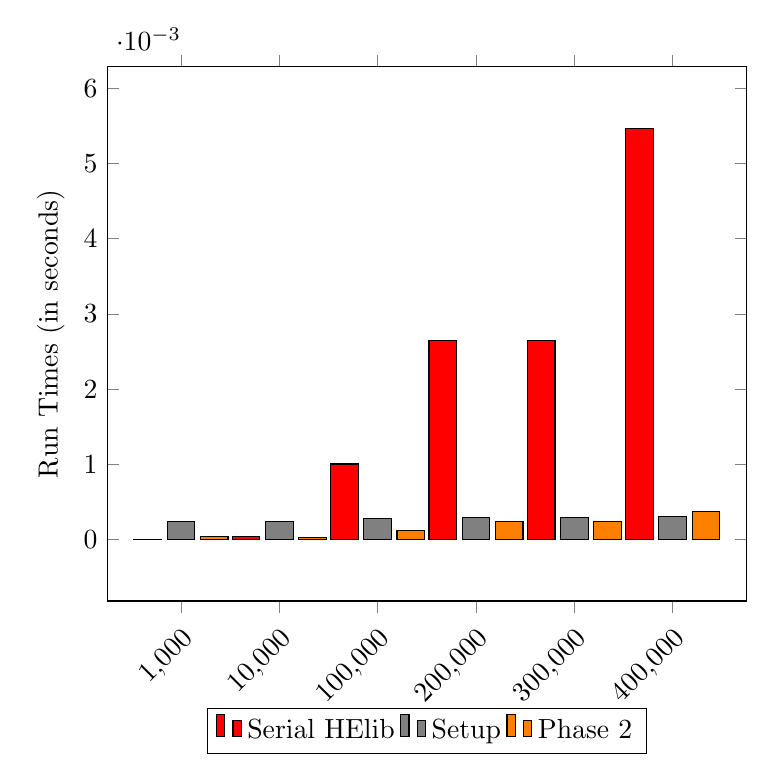
\begin{tikzpicture}

\begin{axis}[
    ybar,
    width=.8\textwidth,
    enlargelimits=0.15,
    legend style={at={(0.5,-0.2)},anchor=north,legend columns=-1},
    ylabel=Run Times (in seconds),
    symbolic x coords={$1{,}000$,$10{,}000$,$100{,}000$,$200{,}000$,$300{,}000$,$400{,}000$},
    xtick=data,
    x tick label style={rotate=45,anchor=north east},
]

\addplot[fill=red]
    coordinates {
    ($1{,}000$,5.000E-06)($10{,}000$,4.825E-05)($100{,}000$,1.007E-03)($200{,}000$,2.648E-03)($300{,}000$,2.653E-03)($400{,}000$,5.466E-03) };
    
\addplot[fill=gray]
    coordinates {
    ($1{,}000$,2.420E-04)($10{,}000$,2.465E-04)($100{,}000$,2.848E-04)($200{,}000$,3.013E-04)($300{,}000$,3.015E-04)($400{,}000$,3.133E-04) };
    
\addplot[fill=orange]
    coordinates {
    ($1{,}000$,4.425E-05)($10{,}000$,3.350E-05)($100{,}000$,1.283E-04)($200{,}000$,2.423E-04)($300{,}000$,2.420E-04)($400{,}000$,3.728E-04) };
    
\legend{Serial HElib,Setup,Phase 2}
\end{axis}
\end{tikzpicture}

\caption{Add Phase Level Run Times Comparison - Operation}
\label{fig:level3ComparisonSerialGPUAddVecs1}
\end{figure}

\begin{figure}[p]
\centering
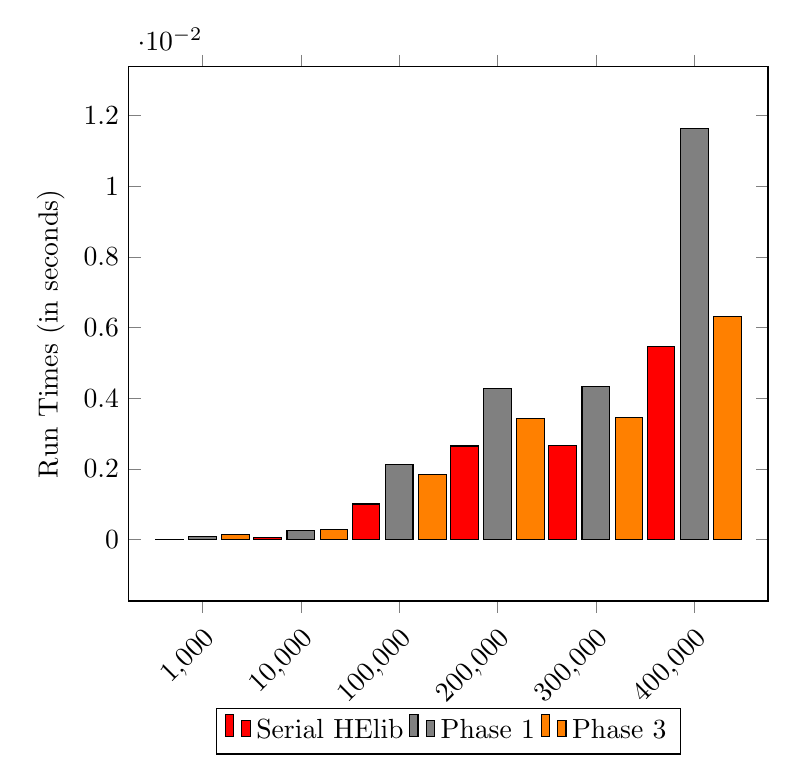
\begin{tikzpicture}

\begin{axis}[
    ybar,
    width=.8\textwidth,
    enlargelimits=0.15,
    legend style={at={(0.5,-0.2)},anchor=north,legend columns=-1},
    ylabel=Run Times (in seconds),
    symbolic x coords={$1{,}000$,$10{,}000$,$100{,}000$,$200{,}000$,$300{,}000$,$400{,}000$},
    xtick=data,
    x tick label style={rotate=45,anchor=north east},
]

\addplot[fill=red]
    coordinates {
    ($1{,}000$,5.000E-06)($10{,}000$,4.825E-05)($100{,}000$,1.007E-03)($200{,}000$,2.648E-03)($300{,}000$,2.653E-03)($400{,}000$,5.466E-03) };
    
\addplot[fill=gray]
    coordinates {
    ($1{,}000$,9.500E-05)($10{,}000$,2.568E-04)($100{,}000$,2.137E-03)($200{,}000$,4.289E-03)($300{,}000$,4.345E-03)($400{,}000$,1.164E-02) };
    
\addplot[fill=orange]
    coordinates {
    ($1{,}000$,1.373E-04)($10{,}000$,2.900E-04)($100{,}000$,1.837E-03)($200{,}000$,3.420E-03)($300{,}000$,3.454E-03)($400{,}000$,6.308E-03) };
    
\legend{Serial HElib,Phase 1,Phase 3}
\end{axis}
\end{tikzpicture}

\caption{Add Phase Level Run Times Comparison - Memory}
\label{fig:level3ComparisonSerialGPUAddVecs2}
\end{figure}

\begin{table}[p]
\centering
\begin{tabular}{ | r | r | r | r | r | r | r | }
 \multicolumn{1}{ r }{} & \multicolumn{6}{ c }{$size\_of\_row$} \\ \cline{2-7}
 \multicolumn{1}{ r |}{} & $1{,}000$ & $10{,}000$ & $100{,}000$ & $200{,}000$ & $300{,}000$ & $400{,}000$ \\ \hline
 Setup & 2.455E-04 & 2.830E-04 & 3.035E-04 & 3.065E-04 & 3.045E-04 & 3.050E-04 \\ \hline
 Phase 1 & 9.000E-05 & 2.535E-04 & 2.262E-03 & 4.377E-03 & 4.377E-03 & 1.152E-02 \\ \hline
 Phase 2 & 3.400E-05 & 4.200E-05 & 1.280E-04 & 2.420E-04 & 2.425E-04 & 3.745E-04 \\ \hline
 Phase 3 & 1.275E-04 & 3.120E-04 & 1.799E-03 & 3.466E-03 & 3.465E-03 & 6.275E-03 \\ \hline
\end{tabular}
\caption{GPUHElib Sub phase level run times (in seconds)}
\label{tab:GPULevel3RuntimesSubVecs}
\end{table}

\begin{figure}[p]
\centering
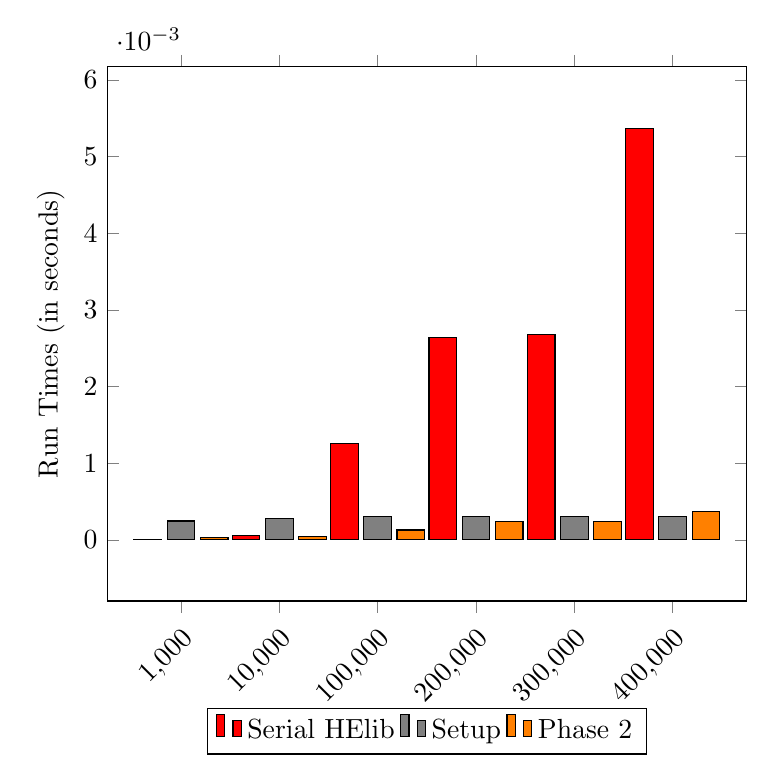
\begin{tikzpicture}

\begin{axis}[
    ybar,
    width=.8\textwidth,
    enlargelimits=0.15,
    legend style={at={(0.5,-0.2)},anchor=north,legend columns=-1},
    ylabel=Run Times (in seconds),
    symbolic x coords={$1{,}000$,$10{,}000$,$100{,}000$,$200{,}000$,$300{,}000$,$400{,}000$},
    xtick=data,
    x tick label style={rotate=45,anchor=north east},
]

\addplot[fill=red]
    coordinates {
    ($1{,}000$,5.000E-06)($10{,}000$,6.150E-05)($100{,}000$,1.259E-03)($200{,}000$,2.644E-03)($300{,}000$,2.674E-03)($400{,}000$,5.366E-03) };
    
\addplot[fill=gray]
    coordinates {
    ($1{,}000$,2.455E-04)($10{,}000$,2.830E-04)($100{,}000$,3.035E-04)($200{,}000$,3.065E-04)($300{,}000$,3.045E-04)($400{,}000$,3.050E-04) };
    
\addplot[fill=orange]
    coordinates {
    ($1{,}000$,3.400E-05)($10{,}000$,4.200E-05)($100{,}000$,1.280E-04)($200{,}000$,2.420E-04)($300{,}000$,2.425E-04)($400{,}000$,3.745E-04) };
    
\legend{Serial HElib,Setup,Phase 2}
\end{axis}
\end{tikzpicture}

\caption{Sub Phase Level Run Times Comparison - Operation}
\label{fig:level3ComparisonSerialGPUSubVecs1}
\end{figure}

\begin{figure}[p]
\centering
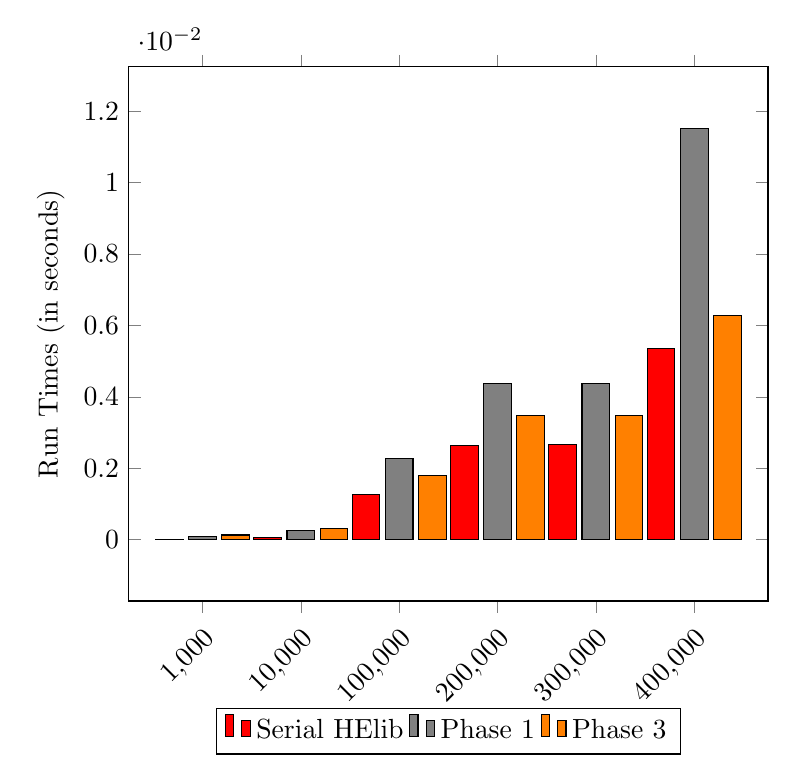
\begin{tikzpicture}

\begin{axis}[
    ybar,
    width=.8\textwidth,
    enlargelimits=0.15,
    legend style={at={(0.5,-0.2)},anchor=north,legend columns=-1},
    ylabel=Run Times (in seconds),
    symbolic x coords={$1{,}000$,$10{,}000$,$100{,}000$,$200{,}000$,$300{,}000$,$400{,}000$},
    xtick=data,
    x tick label style={rotate=45,anchor=north east},
]

\addplot[fill=red]
    coordinates {
    ($1{,}000$,5.000E-06)($10{,}000$,6.150E-05)($100{,}000$,1.259E-03)($200{,}000$,2.644E-03)($300{,}000$,2.674E-03)($400{,}000$,5.366E-03) };
    
\addplot[fill=gray]
    coordinates {
    ($1{,}000$,9.000E-05)($10{,}000$,2.535E-04)($100{,}000$,2.262E-03)($200{,}000$,4.377E-03)($300{,}000$,4.377E-03)($400{,}000$,1.152E-02) };
    
\addplot[fill=orange]
    coordinates {
    ($1{,}000$,1.275E-04)($10{,}000$,3.120E-04)($100{,}000$,1.799E-03)($200{,}000$,3.466E-03)($300{,}000$,3.465E-03)($400{,}000$,6.275E-03) };
    
\legend{Serial HElib,Phase 1,Phase 3}
\end{axis}
\end{tikzpicture}

\caption{Sub Phase Level Run Times Comparison - Memory}
\label{fig:level3ComparisonSerialGPUSubVecs2}
\end{figure}

\begin{table}[p]
\centering
\begin{tabular}{ | r | r | r | r | r | r | r | }
 \multicolumn{1}{ r }{} & \multicolumn{6}{ c }{$size\_of\_row$} \\ \cline{2-7}
 \multicolumn{1}{ r |}{} & $1{,}000$ & $10{,}000$ & $100{,}000$ & $200{,}000$ & $300{,}000$ & $400{,}000$ \\ \hline
 Setup & 2.405E-04 & 2.447E-04 & 3.027E-04 & 3.200E-04 & 3.157E-04 & 3.207E-04 \\ \hline
 Phase 1 & 7.933E-05 & 1.853E-04 & 1.845E-03 & 3.955E-03 & 3.997E-03 & 1.029E-02 \\ \hline
 Phase 2 & 3.000E-05 & 3.183E-05 & 1.247E-04 & 2.398E-04 & 2.353E-04 & 3.508E-04 \\ \hline
 Phase 3 & 1.772E-04 & 5.418E-04 & 4.323E-03 & 8.213E-03 & 8.212E-03 & 1.591E-02 \\ \hline
\end{tabular}
\caption{GPUHElib Mul phase level run times (in seconds)}
\label{tab:GPULevel3RuntimesMulVecs}
\end{table}

\begin{figure}[p]
\centering
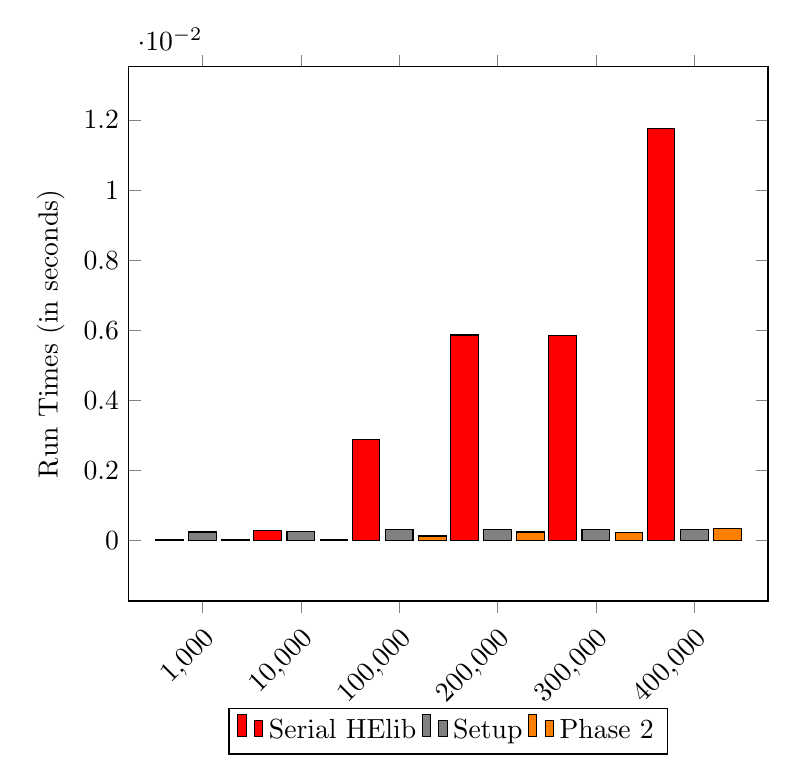
\begin{tikzpicture}

\begin{axis}[
    ybar,
    width=.8\textwidth,
    enlargelimits=0.15,
    legend style={at={(0.5,-0.2)},anchor=north,legend columns=-1},
    ylabel=Run Times (in seconds),
    symbolic x coords={$1{,}000$,$10{,}000$,$100{,}000$,$200{,}000$,$300{,}000$,$400{,}000$},
    xtick=data,
    x tick label style={rotate=45,anchor=north east},
]

\addplot[fill=red]
    coordinates {
    ($1{,}000$,2.900E-05)($10{,}000$,2.830E-04)($100{,}000$,2.879E-03)($200{,}000$,5.863E-03)($300{,}000$,5.856E-03)($400{,}000$,1.176E-02) };
    
\addplot[fill=gray]
    coordinates {
    ($1{,}000$,2.405E-04)($10{,}000$,2.447E-04)($100{,}000$,3.027E-04)($200{,}000$,3.200E-04)($300{,}000$,3.157E-04)($400{,}000$,3.207E-04) };
    
\addplot[fill=orange]
    coordinates {
    ($1{,}000$,3.000E-05)($10{,}000$,3.183E-05)($100{,}000$,1.247E-04)($200{,}000$,2.398E-04)($300{,}000$,2.353E-04)($400{,}000$,3.508E-04) };
    
\legend{Serial HElib,Setup,Phase 2}
\end{axis}
\end{tikzpicture}

\caption{Mul Phase Level Run Times Comparison - Operation}
\label{fig:level3ComparisonSerialGPUMulVecs1}
\end{figure}

\begin{figure}[p]
\centering
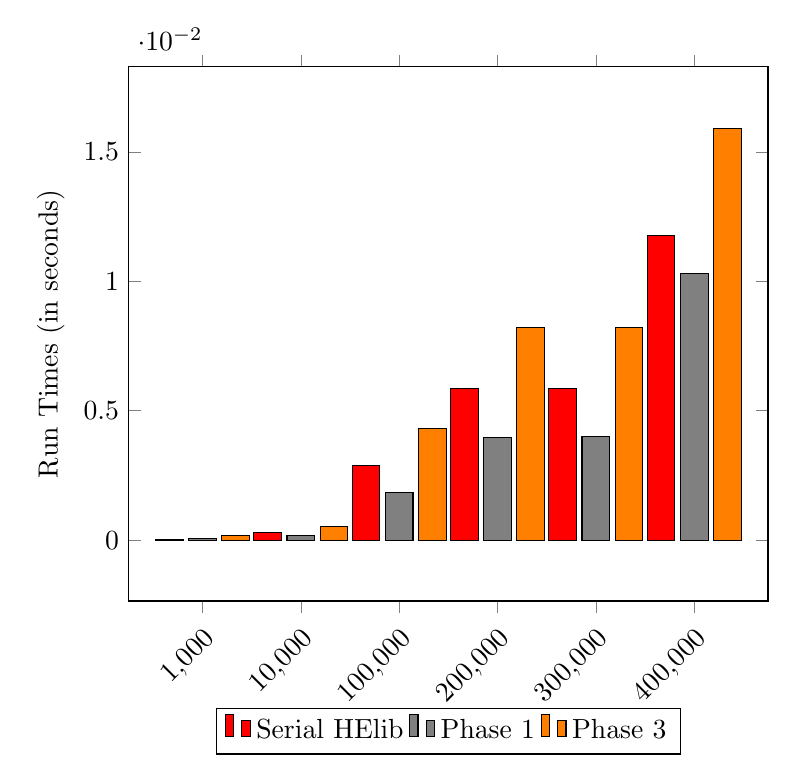
\begin{tikzpicture}

\begin{axis}[
    ybar,
    width=.8\textwidth,
    enlargelimits=0.15,
    legend style={at={(0.5,-0.2)},anchor=north,legend columns=-1},
    ylabel=Run Times (in seconds),
    symbolic x coords={$1{,}000$,$10{,}000$,$100{,}000$,$200{,}000$,$300{,}000$,$400{,}000$},
    xtick=data,
    x tick label style={rotate=45,anchor=north east},
]

\addplot[fill=red]
    coordinates {
    ($1{,}000$,2.900E-05)($10{,}000$,2.830E-04)($100{,}000$,2.879E-03)($200{,}000$,5.863E-03)($300{,}000$,5.856E-03)($400{,}000$,1.176E-02) };
    
\addplot[fill=gray]
    coordinates {
    ($1{,}000$,7.933E-05)($10{,}000$,1.853E-04)($100{,}000$,1.845E-03)($200{,}000$,3.955E-03)($300{,}000$,3.997E-03)($400{,}000$,1.029E-02) };
    
\addplot[fill=orange]
    coordinates {
    ($1{,}000$,1.772E-04)($10{,}000$,5.418E-04)($100{,}000$,4.323E-03)($200{,}000$,8.213E-03)($300{,}000$,8.212E-03)($400{,}000$,1.591E-02) };
    
\legend{Serial HElib,Phase 1,Phase 3}
\end{axis}
\end{tikzpicture}

\caption{Mul Phase Level Run Times Comparison - Memory}
\label{fig:level3ComparisonSerialGPUMulVecs2}
\end{figure}

Table \ref{tab:GPULevel3RuntimesAddVecs}, Table \ref{tab:GPULevel3RuntimesSubVecs}, and Table \ref{tab:GPULevel3RuntimesMulVecs} all display the phase level run times for each operation respectively. The four phases are: setup (vector and stream creation), phase 1 (host to device memory copy), phase 2 (operation on GPU), and phase 3 (device to host memory copy). These times have been split between two plots for each operation. One group of plots focuses on the overall run time of serial HElib compared to the setup and phase 2 times recorded. These are the \say{Operation} plots, Figure \ref{fig:level3ComparisonSerialGPUAddVecs1}, Figure \ref{fig:level3ComparisonSerialGPUSubVecs1}, and Figure \ref{fig:level3ComparisonSerialGPUMulVecs1}. The other group of plots focus on the overhead phases, phase 1 and phase 3, of GPUHElib compared to the overall run time of serial HElib for each operation and are denoted \say{Memory}. These are Figure \ref{fig:level3ComparisonSerialGPUAddVecs2}, Figure \ref{fig:level3ComparisonSerialGPUSubVecs2}, and Figure \ref{fig:level3ComparisonSerialGPUMulVecs2}.

The \say{Operation} plots show that the design is working as intended and as all GPU designs are ideally suppose to work. The reliance on the GPU to perform the computation drastically reduces the run time for those phases. Furthermore, as the input size increases largely, the run times for setup and phase 2 only increase slightly. 

The setup phase always took about the same amount of time no matter the input size, only varying by about 8E-05 from the smallest input to the largest. Phase 2 times steadily increased, however not at the rapid pace of the serial HElib versions. This is what is expected when using a GPU to perform operations.

These are the desired results when working with a GPU. The offloading of work onto the GPU allows for the operation portions of the work to drastically decrease in run time. Of course, these results do not characterize the overall recorded times for GPUHElib compared to serial HElib. Therefore something else must be going wrong, that is causing the run times to be longer than the their serial counterparts.

The \say{Memory} plots show where this design fails. The amount of time needed to move the data back and forth from the GPU is immense. The times for phase 1 and phase 3 are always larger than the entire run time of the serial version for every operation across all input sizes, except for the multiplication operation, where the phase 1 times are actually less than the overall run time of the serial version, but not by much. These times are very disappointing, as they are the reason that this design is performing so poorly. Luckily, these times could be lower, given better hardware and possible future work, which could make GPUHElib a viable option. If the problem was in the design or if the run times for the setup or phase 1 were worse, then the total design would not have any hope of being used. But because they are in the memory transfer phases, there is still hope that this design could become viable with further work.

\section{DistrubtedHElib Evaluation Results} \label{sec:DistributedHElibEvaluationResults}
As discussed earlier in this chapter, DistributedHElib has three levels of timing information begin recorded. The highest level is the circuit level in the test program. The next is at the function level, inside \verb|DoubleCRT|. The third and lowest level is the distribute and wait level. This level has two timers which measure the distribute time, the time necessary for the dispatcher node to assign work and partition the data, and the wait time, the time the dispatcher node is waiting for the compute nodes to finish their work and return the results. Additionally three cluster sizes, 4, 8, and 16 nodes, were used during testing The timing results for each of these levels is discussed in more detail below.

\subsection{DistributedHElib Circuit Level Run Times}
\begin{table}[p]
\centering
\begin{tabular}{ | r | r | r | r | r | r | r | }
 \multicolumn{1}{ r }{} & \multicolumn{6}{ c }{$size\_of\_row$} \\ \cline{2-7}
 \multicolumn{1}{ r |}{} & $1{,}000$ & $10{,}000$ & $100{,}000$ & $200{,}000$ & $300{,}000$ & $400{,}000$ \\ \hline
 Add & 1.400E-05 & 1.070E-04 & 2.525E-03 & 5.347E-03 & 5.313E-03 & 1.048E-02 \\ \hline
 Sub & 1.400E-05 & 1.250E-04 & 2.491E-03 & 5.308E-03 & 5.244E-03 & 1.080E-02 \\ \hline
 Mul & 4.996E-03 & 1.030E-01 & 1.151 & 2.644 & 7.286 & 1.202E+01 \\ \hline
\end{tabular}
\caption{Serial HElib circuit level run times (in seconds)}
\label{tab:DistributedserialLevel1Runtimes}
\end{table}

\begin{table}[p]
\centering
\begin{tabular}{ | r | r | r | r | r | r | r | }
 \multicolumn{1}{ r }{} & \multicolumn{6}{ c }{$size\_of\_row$} \\ \cline{2-7}
 \multicolumn{1}{ r |}{} & $1{,}000$ & $10{,}000$ & $100{,}000$ & $200{,}000$ & $300{,}000$ & $400{,}000$ \\ \hline
 Add & 1.457E-03 & 7.496E-03 & 8.933E-02 & 1.783E-01 & 1.550E-01 & 3.455E-01 \\ \hline
 Sub & 1.544E-03 & 7.479E-03 & 7.773E-02 & 1.666E-01 & 1.647E-01 & 3.203E-01 \\ \hline
 Mul & 1.254E-02 & 1.371E-01 & 1.559 & 3.444 & 8.350 & 1.009E+01 \\ \hline
\end{tabular}
\caption{DistributedHElib circuit level run times (in seconds) on 4 nodes}
\label{tab:DistributedLevel1Runtimes4Nodes}
\end{table}

\begin{figure}[p]
\centering

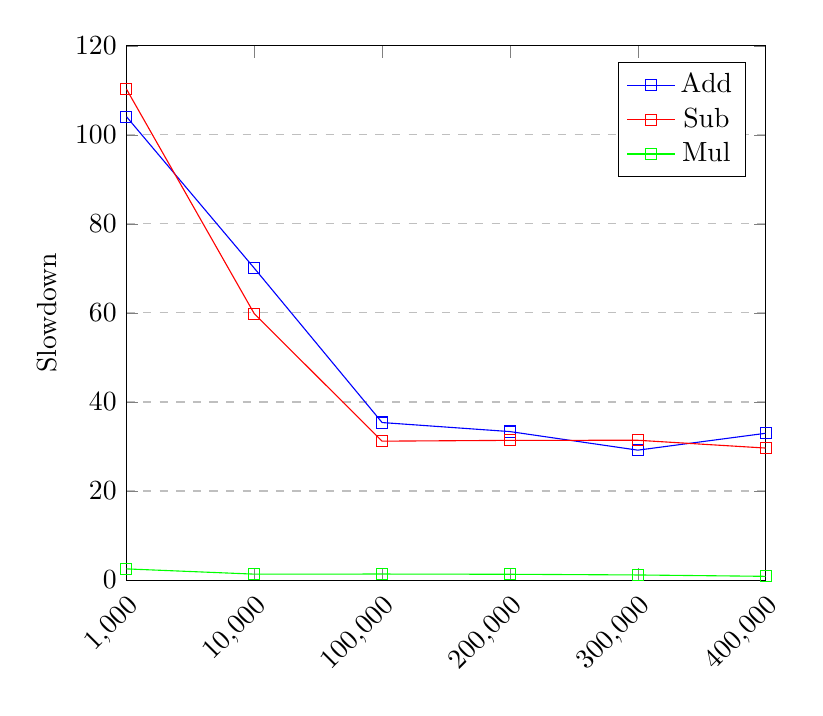
\begin{tikzpicture}
\begin{axis}
[
    ylabel={Slowdown},
    width=.8\textwidth,
    xmin=1, xmax=6,
    ymin=0, ymax=120,
    xtick={1,2,3,4,5,6},
    xticklabels={$1{,}000$, $10{,}000$, $100{,}000$, $200{,}000$, $300{,}000$, $400{,}000$},
    ytick={120,100,80,60,40,20,0},
    legend pos=north east,
    ymajorgrids=true,
    grid style=dashed,
    x tick label style={rotate=45,anchor=north east},
]

\addplot[color=blue,mark=square]
    coordinates {
    (1,1.041E+02)(2,7.006E+01)(3,3.538E+01)(4,3.335E+01)(5,2.918E+01)(6,3.297E+01) };
    
\addplot[color=red,mark=square]
    coordinates {
    (1,1.103E+02)(2,5.983E+01)(3,3.120E+01)(4,3.138E+01)(5,3.140E+01)(6,2.965E+01) };

\addplot[color=green,mark=square]
    coordinates {
    (1,2.510E+00)(2,1.332E+00)(3,1.354E+00)(4,1.302E+00)(5,1.146E+00)(6,8.393E-01) };
    
\legend{Add,Sub,Mul}
 
\end{axis}
\end{tikzpicture}

\caption{Run Time Comparison at Circuit Level on 4 Nodes}
\label{fig:level1ComparisonSerialDistributed4Nodes}
\end{figure}

\begin{table}[p]
\centering
\begin{tabular}{ | r | r | r | r | r | r | r | }
 \multicolumn{1}{ r }{} & \multicolumn{6}{ c }{$size\_of\_row$} \\ \cline{2-7}
 \multicolumn{1}{ r |}{} & $1{,}000$ & $10{,}000$ & $100{,}000$ & $200{,}000$ & $300{,}000$ & $400{,}000$ \\ \hline
 Add & 1.712E-03 & 9.161E-03 & 1.076E-01 & 2.228E-01 & 2.266E-01 & 4.540E-01 \\ \hline
 Sub & 1.791E-03 & 9.219E-03 & 1.117E-01 & 2.113E-01 & 2.139E-01 & 4.560E-01 \\ \hline
 Mul & 1.350E-02 & 1.454E-01 & 1.666 & 3.689 & 8.589 & 1.136E+01 \\ \hline
\end{tabular}
\caption{DistributedHElib circuit level run times (in seconds) on 8 nodes}
\label{tab:DistributedLevel1Runtimes8Nodes}
\end{table}

\begin{figure}[p]
\centering

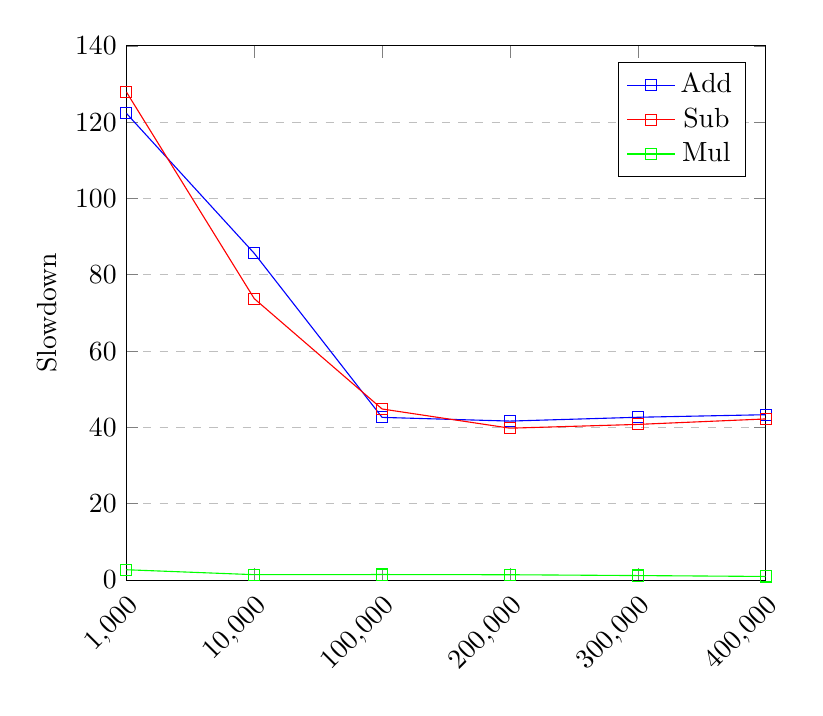
\begin{tikzpicture}
\begin{axis}
[
    ylabel={Slowdown},
    width=.8\textwidth,
    xmin=1, xmax=6,
    ymin=0, ymax=140,
    xtick={1,2,3,4,5,6},
    xticklabels={$1{,}000$, $10{,}000$, $100{,}000$, $200{,}000$, $300{,}000$, $400{,}000$},
    ytick={140,120,100,80,60,40,20,0},
    legend pos=north east,
    ymajorgrids=true,
    grid style=dashed,
    x tick label style={rotate=45,anchor=north east},
]

\addplot[color=blue,mark=square]
    coordinates {
    (1,1.223E+02)(2,8.562E+01)(3,4.263E+01)(4,4.166E+01)(5,4.266E+01)(6,4.333E+01) };
    
\addplot[color=red,mark=square]
    coordinates {
    (1,1.279E+02)(2,7.375E+01)(3,4.483E+01)(4,3.980E+01)(5,4.079E+01)(6,4.222E+01) };

\addplot[color=green,mark=square]
    coordinates {
    (1,2.703E+00)(2,1.412E+00)(3,1.447E+00)(4,1.395E+00)(5,1.179E+00)(6,9.451E-01) };
    
\legend{Add,Sub,Mul}
 
\end{axis}
\end{tikzpicture}

\caption{Run Time Comparison at Circuit Level on 8 Nodes}
\label{fig:level1ComparisonSerialDistributed8Nodes}
\end{figure}

\begin{table}[p]
\centering
\begin{tabular}{ | r | r | r | r | r | r | r | }
 \multicolumn{1}{ r }{} & \multicolumn{6}{ c }{$size\_of\_row$} \\ \cline{2-7}
 \multicolumn{1}{ r |}{} & $1{,}000$ & $10{,}000$ & $100{,}000$ & $200{,}000$ & $300{,}000$ & $400{,}000$ \\ \hline
 Add & 1.772E-03 & 9.960E-03 & 1.187E-01 & 2.391E-01 & 2.390E-01 & 4.911E-01 \\ \hline
 Sub & 1.850E-03 & 9.741E-03 & 1.194E-01 & 2.398E-01 & 2.364E-01 & 4.744E-01 \\ \hline
 Mul & 2.484E-02 & 1.623E-01 & 1.717 & 3.811 & 8.664 & 1.135E+01 \\ \hline
\end{tabular}
\caption{DistributedHElib circuit level run times (in seconds) on 16 nodes}
\label{tab:DistributedLevel1Runtimes16Nodes}
\end{table}

\begin{figure}[p]
\centering

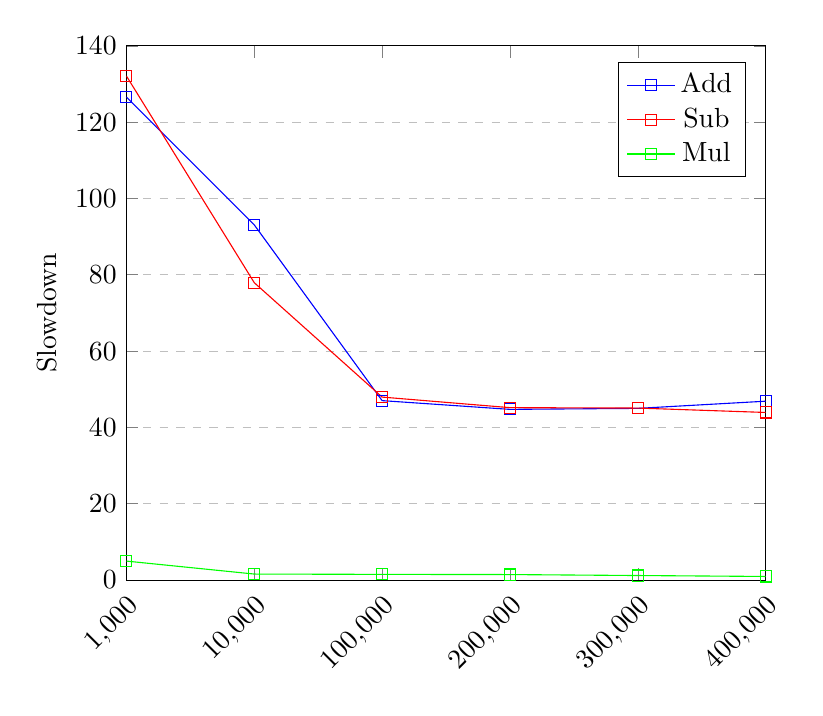
\begin{tikzpicture}
\begin{axis}
[
    ylabel={Slowdown},
    width=.8\textwidth,
    xmin=1, xmax=6,
    ymin=0, ymax=140,
    xtick={1,2,3,4,5,6},
    xticklabels={$1{,}000$, $10{,}000$, $100{,}000$, $200{,}000$, $300{,}000$, $400{,}000$},
    ytick={140,120,100,80,60,40,20,0},
    legend pos=north east,
    ymajorgrids=true,
    grid style=dashed,
    x tick label style={rotate=45,anchor=north east},
]

\addplot[color=blue,mark=square]
    coordinates {
    (1,1.266E+02)(2,9.308E+01)(3,4.702E+01)(4,4.473E+01)(5,4.499E+01)(6,4.687E+01) };
    
\addplot[color=red,mark=square]
    coordinates {
    (1,1.321E+02)(2,7.793E+01)(3,4.795E+01)(4,4.518E+01)(5,4.507E+01)(6,4.392E+01) };

\addplot[color=green,mark=square]
    coordinates {
    (1,4.971E+00)(2,1.576E+00)(3,1.491E+00)(4,1.441E+00)(5,1.189E+00)(6,9.438E-01) };
    
\legend{Add,Sub,Mul}
 
\end{axis}
\end{tikzpicture}

\caption{Run Time Comparison at Circuit Level on 16 Nodes}
\label{fig:level1ComparisonSerialDistributed16Nodes}
\end{figure}

Table \ref{tab:DistributedserialLevel1Runtimes}, Table \ref{tab:DistributedLevel1Runtimes4Nodes}, Table \ref{tab:DistributedLevel1Runtimes8Nodes}, and Table \ref{tab:DistributedLevel1Runtimes16Nodes} display the run times for serial HElib and DistributedHElib tests. Both tests were run with inputs sizes starting at 1,000 and increasing until 400,000. The clusters sizes were 4, 8, and 16 nodes.

Figure \ref{fig:level1ComparisonSerialDistributed4Nodes}, Figure \ref{fig:level1ComparisonSerialDistributed8Nodes}, and Figure \ref{fig:level1ComparisonSerialDistributed16Nodes} visualize these times as the slowdown of DistributedHElib over serial HElib. A value of 1 means that the serial version and the distributed version had the same run time. Above 1 means that the distributed design has a slower run time, and below 1 means that the distributed version has a faster run time.

One can see in these figures that for the smaller input sizes, the run times for addition and subtraction across all cluster sizes are much larger for the distributed design compared to the serial design. These operations take over 100 times as long to complete as their serial counterparts. The multiplication operation also takes longer, however only about 2.5 to 5 times as long depending on the number of nodes in the cluster. 

As the input sizes increase, the addition and subtraction operation slowdowns decrease, until they plateau at around 35, 40, and 45 times as long for the 4, 8, and 16 node clusters respectively. Once they reach these slowdowns, they bounce around them, but never continue on the downward trajectory they had for the first few input size increases. The multiplication operation on the other hand always decreases as the input size increases. As the input sizes increase, the multiplication slowdowns approach 1, and at the 400,000 size input, all three cluster sizes dive below 1. The cluster size of 4 has the best results, having about a .84 slowdown, with the other two sizes, 8 and 16, having about a .94. These results mean that for the 400,000 input size the distributed variant of HElib had faster run times than the serial version across all cluster sizes. Similar to the GPU results however, while these times look good, further examination of the lower level tests show that this speed up is probably not happening because of the distributed design, but because of other factors. Next the function level times are examined.

\subsection{DistributedHElib Function Level Run Times}
\begin{table}[p]
\centering
\begin{tabular}{ | r | r | r | r | r | r | r | }
 \multicolumn{1}{ r }{} & \multicolumn{6}{ c }{$size\_of\_row$} \\ \cline{2-7}
 \multicolumn{1}{ r |}{} & $1{,}000$ & $10{,}000$ & $100{,}000$ & $200{,}000$ & $300{,}000$ & $400{,}000$ \\ \hline
 Add & 5.000E-06 & 4.800E-05 & 9.873E-04 & 2.588E-03 & 2.611E-03 & 5.457E-03 \\ \hline
 Sub & 5.000E-06 & 5.850E-05 & 1.238E-03 & 2.646E-03 & 2.614E-03 & 5.391E-03 \\ \hline
 Mul & 2.967E-05 & 2.838E-04 & 2.887E-03 & 5.845E-03 & 5.850E-03 & 1.183E-02 \\ \hline
\end{tabular}
\caption{Serial HElib function level run times (in seconds)}
\label{tab:DistributedserialLevel2Runtimes}
\end{table}

\begin{table}[p]
\centering
\begin{tabular}{ | r | r | r | r | r | r | r | }
 \multicolumn{1}{ r }{} & \multicolumn{6}{ c }{$size\_of\_row$} \\ \cline{2-7}
 \multicolumn{1}{ r |}{} & $1{,}000$ & $10{,}000$ & $100{,}000$ & $200{,}000$ & $300{,}000$ & $400{,}000$ \\ \hline
 Add & 7.423E-04 & 3.604E-03 & 4.898E-02 & 8.503E-02 & 8.048E-02 & 1.764E-01 \\ \hline
 Sub & 7.695E-04 & 3.735E-03 & 3.886E-02 & 8.329E-02 & 8.233E-02 & 1.601E-01 \\ \hline
 Mul & 7.148E-04 & 3.298E-03 & 3.517E-02 & 7.759E-02 & 7.771E-02 & 1.482E-01 \\ \hline
\end{tabular}
\caption{DistributedHElib function level run times (in seconds) on 4 nodes}
\label{tab:DistributedLevel2Runtimes4Nodes}
\end{table}

\begin{table}[p]
\centering
\begin{tabular}{ | r | r | r | r | r | r | r | }
 \multicolumn{1}{ r }{} & \multicolumn{6}{ c }{$size\_of\_row$} \\ \cline{2-7}
 \multicolumn{1}{ r |}{} & $1{,}000$ & $10{,}000$ & $100{,}000$ & $200{,}000$ & $300{,}000$ & $400{,}000$ \\ \hline
 Add & 8.698E-04 & 4.427E-03 & 5.489E-02 & 1.124E-01 & 1.125E-01 & 2.186E-01 \\ \hline
 Sub & 8.930E-04 & 4.427E-03 & 5.583E-02 & 1.056E-01 & 1.069E-01 & 2.280E-01 \\ \hline
 Mul & 8.055E-04 & 4.032E-03 & 4.830E-02 & 9.798E-02 & 9.804E-02 & 1.951E-01 \\ \hline
\end{tabular}
\caption{DistributedHElib function level run times (in seconds) on 8 nodes}
\label{tab:DistributedLevel2Runtimes8Nodes}
\end{table}

\begin{table}[p]
\centering
\begin{tabular}{ | r | r | r | r | r | r | r | }
 \multicolumn{1}{ r }{} & \multicolumn{6}{ c }{$size\_of\_row$} \\ \cline{2-7}
 \multicolumn{1}{ r |}{} & $1{,}000$ & $10{,}000$ & $100{,}000$ & $200{,}000$ & $300{,}000$ & $400{,}000$ \\ \hline
 Add & 9.180E-04 & 7.439E-03 & 5.794E-02 & 1.166E-01 & 1.152E-01 & 2.316E-01 \\ \hline
 Sub & 9.220E-04 & 4.866E-03 & 5.971E-02 & 1.199E-01 & 1.182E-01 & 2.372E-01 \\ \hline
 Mul & 8.373E-04 & 4.498E-03 & 5.036E-02 & 1.025E-01 & 1.054E-01 & 2.126E-01 \\ \hline
\end{tabular}
\caption{DistributedHElib function level run times (in seconds) on 16 nodes}
\label{tab:DistributedLevel2Runtimes16Nodes}
\end{table}

\begin{figure}[p]
\centering
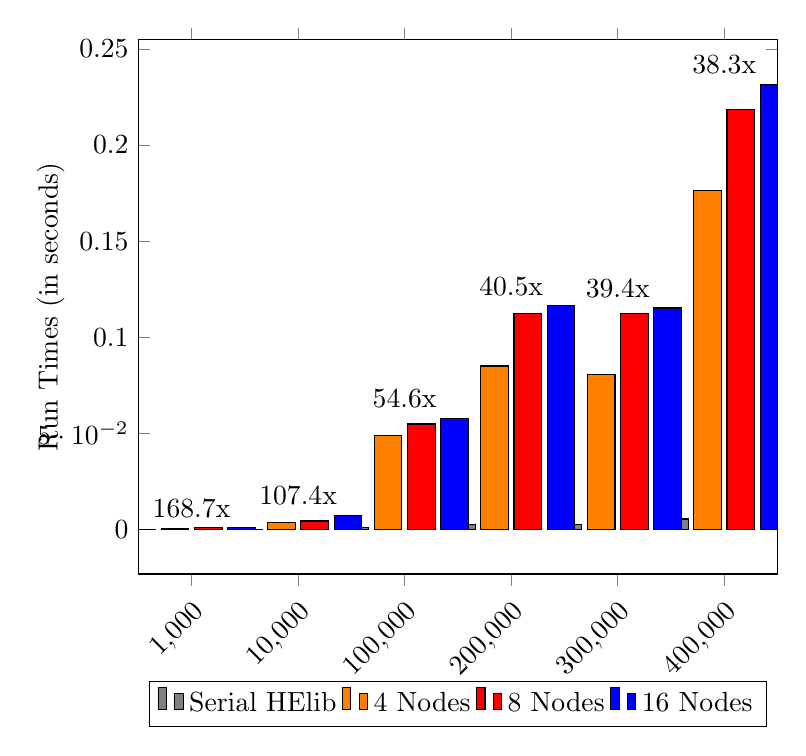
\begin{tikzpicture}

\begin{axis}[
    ybar,
    width=.8\textwidth,
    legend style={at={(0.5,-0.2)},anchor=north,legend columns=-1},
    ylabel=Run Times (in seconds),
    symbolic x coords={$1{,}000$,$10{,}000$,$100{,}000$,$200{,}000$,$300{,}000$,$400{,}000$},
    xtick=data,
    x tick label style={rotate=45,anchor=north east},
    y label style={at={(axis description cs:-0.1,0.5)}, anchor=south},
]

\addplot[fill=gray]
    coordinates {
    ($1{,}000$,5.000E-06)($10{,}000$,4.800E-05)($100{,}000$,9.873E-04)($200{,}000$,2.588E-03)($300{,}000$,2.611E-03)($400{,}000$,5.457E-03) };
    
\addplot[fill=orange]
    coordinates {
    ($1{,}000$,7.423E-04)($10{,}000$,3.604E-03)($100{,}000$,4.898E-02)($200{,}000$,8.503E-02)($300{,}000$,8.048E-02)($400{,}000$,1.764E-01) };
    
\addplot[fill=red]
    coordinates {
    ($1{,}000$,8.698E-04)($10{,}000$,4.427E-03)($100{,}000$,5.489E-02)($200{,}000$,1.124E-01)($300{,}000$,1.125E-01)($400{,}000$,2.186E-01) };
    
\addplot[fill=blue]
    coordinates {
    ($1{,}000$,9.180E-04)($10{,}000$,7.439E-03)($100{,}000$,5.794E-02)($200{,}000$,1.166E-01)($300{,}000$,1.152E-01)($400{,}000$,2.316E-01) };

\node at (axis cs:$1{,}000$,1.092E-02) {168.7x};
\node at (axis cs:$10{,}000$,1.744E-02) {107.4x};
\node at (axis cs:$100{,}000$,6.794E-02) {54.6x};
\node at (axis cs:$200{,}000$,1.266E-01) {40.5x};
\node at (axis cs:$300{,}000$,1.252E-01) {39.4x};
\node at (axis cs:$400{,}000$,2.416E-01) {38.3x};
    
\legend{Serial HElib,4 Nodes,8 Nodes,16 Nodes}
\end{axis}
\end{tikzpicture}

\caption{Add Run Times Comparison at Function Level}
\label{fig:level2ComparisonSerialDistributedAddVecs}
\end{figure}

\begin{figure}[p]
\centering
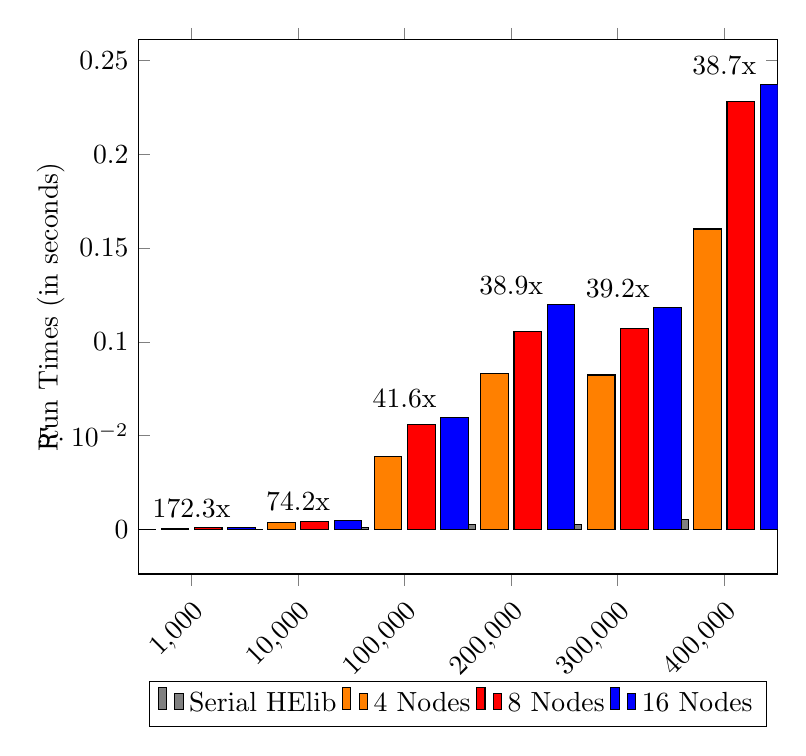
\begin{tikzpicture}

\begin{axis}[
    ybar,
    width=.8\textwidth,
    legend style={at={(0.5,-0.2)},anchor=north,legend columns=-1},
    ylabel=Run Times (in seconds),
    symbolic x coords={$1{,}000$,$10{,}000$,$100{,}000$,$200{,}000$,$300{,}000$,$400{,}000$},
    xtick=data,
    x tick label style={rotate=45,anchor=north east},
    y label style={at={(axis description cs:-0.1,0.5)}, anchor=south},
]

\addplot[fill=gray]
    coordinates {
    ($1{,}000$,5.000E-06)($10{,}000$,5.850E-05)($100{,}000$,1.238E-03)($200{,}000$,2.646E-03)($300{,}000$,2.614E-03)($400{,}000$,5.391E-03) };
    
\addplot[fill=orange]
    coordinates {
    ($1{,}000$,7.695E-04)($10{,}000$,3.735E-03)($100{,}000$,3.886E-02)($200{,}000$,8.329E-02)($300{,}000$,8.233E-02)($400{,}000$,1.601E-01) };
    
\addplot[fill=red]
    coordinates {
    ($1{,}000$,8.930E-04)($10{,}000$,4.427E-03)($100{,}000$,5.583E-02)($200{,}000$,1.056E-01)($300{,}000$,1.069E-01)($400{,}000$,2.280E-01) };
    
\addplot[fill=blue]
    coordinates {
    ($1{,}000$,9.220E-04)($10{,}000$,4.866E-03)($100{,}000$,5.971E-02)($200{,}000$,1.199E-01)($300{,}000$,1.182E-01)($400{,}000$,2.372E-01) };
    
\node at (axis cs:$1{,}000$,1.092E-02) {172.3x};
\node at (axis cs:$10{,}000$,1.487E-02) {74.2x};
\node at (axis cs:$100{,}000$,6.971E-02) {41.6x};
\node at (axis cs:$200{,}000$,1.299E-01) {38.9x};
\node at (axis cs:$300{,}000$,1.282E-01) {39.2x};
\node at (axis cs:$400{,}000$,2.472E-01) {38.7x};
    
\legend{Serial HElib,4 Nodes,8 Nodes,16 Nodes}
\end{axis}
\end{tikzpicture}

\caption{Sub Run Times Comparison at Function Level}
\label{fig:level2ComparisonSerialDistributedSubVecs}
\end{figure}

\begin{figure}[p]
\centering
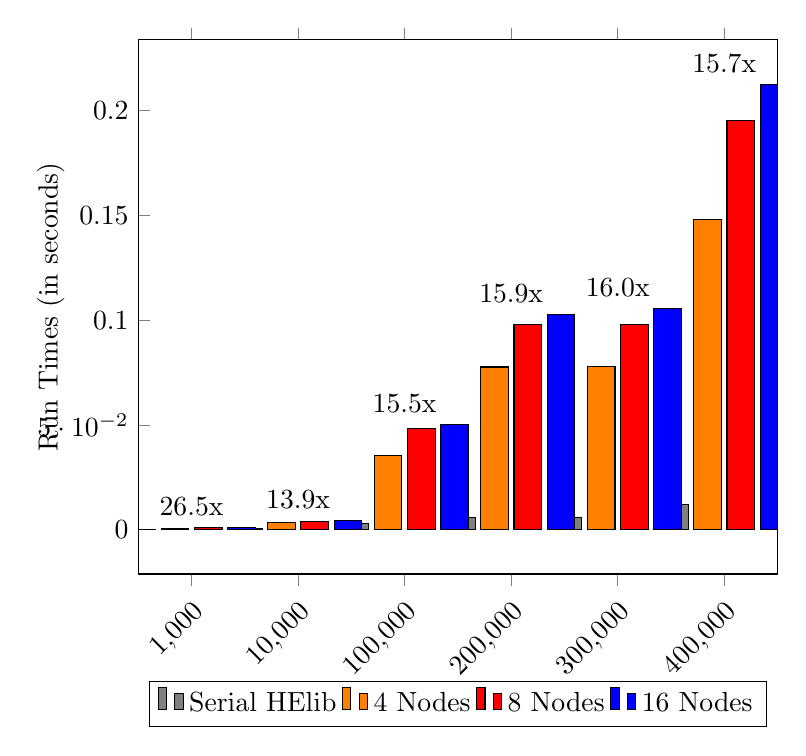
\begin{tikzpicture}

\begin{axis}[
    ybar,
    width=.8\textwidth,
    legend style={at={(0.5,-0.2)},anchor=north,legend columns=-1},
    ylabel=Run Times (in seconds),
    symbolic x coords={$1{,}000$,$10{,}000$,$100{,}000$,$200{,}000$,$300{,}000$,$400{,}000$},
    xtick=data,
    x tick label style={rotate=45,anchor=north east},
    y label style={at={(axis description cs:-0.1,0.5)}, anchor=south},
]

\addplot[fill=gray]
    coordinates {
    ($1{,}000$,2.967E-05)($10{,}000$,2.838E-04)($100{,}000$,2.887E-03)($200{,}000$,5.845E-03)($300{,}000$,5.850E-03)($400{,}000$,1.183E-02) };
    
\addplot[fill=orange]
    coordinates {
    ($1{,}000$,7.148E-04)($10{,}000$,3.298E-03)($100{,}000$,3.517E-02)($200{,}000$,7.759E-02)($300{,}000$,7.771E-02)($400{,}000$,1.482E-01) };
    
\addplot[fill=red]
    coordinates {
    ($1{,}000$,8.055E-04)($10{,}000$,4.032E-03)($100{,}000$,4.830E-02)($200{,}000$,9.798E-02)($300{,}000$,9.804E-02)($400{,}000$,1.951E-01) };
    
\addplot[fill=blue]
    coordinates {
    					
    ($1{,}000$,8.373E-04)($10{,}000$,4.498E-03)($100{,}000$,5.036E-02)($200{,}000$,1.025E-01)($300{,}000$,1.054E-01)($400{,}000$,2.126E-01) };
    
    2.649E+01	1.389E+01	1.545E+01	1.586E+01	1.602E+01	1.566E+01
\node at (axis cs:$1{,}000$,1.084E-02) {26.5x};
\node at (axis cs:$10{,}000$,1.450E-02) {13.9x};
\node at (axis cs:$100{,}000$,6.036E-02) {15.5x};
\node at (axis cs:$200{,}000$,1.125E-01) {15.9x};
\node at (axis cs:$300{,}000$,1.154E-01) {16.0x};
\node at (axis cs:$400{,}000$,2.226E-01) {15.7x};
    
\legend{Serial HElib,4 Nodes,8 Nodes,16 Nodes}
\end{axis}
\end{tikzpicture}

\caption{Mul Run Times Comparison at Function Level}
\label{fig:level2ComparisonSerialDistributedMulVecs}
\end{figure}

Table \ref{tab:DistributedserialLevel2Runtimes}, Table \ref{tab:DistributedLevel2Runtimes4Nodes}, Table \ref{tab:DistributedLevel2Runtimes8Nodes}, and Table \ref{tab:DistributedLevel2Runtimes16Nodes} display the run times at the function level for serial HElib and DistributedHElib on 4, 8, and 16 nodes. 

Figure \ref{fig:level2ComparisonSerialDistributedAddVecs}, Figure \ref{fig:level2ComparisonSerialDistributedSubVecs}, and Figure \ref{fig:level2ComparisonSerialDistributedMulVecs} show the comparisons between the run times for each of the operations at the function level across all variants and cluster sizes. Also displayed in the figures is the average run time slow down, across all cluster sizes, of the distributed variant compared to the serial version. So, for example, in Figure \ref{fig:level2ComparisonSerialDistributedAddVecs}, the 168.7x above 1,000 means that the distributed variant took 168.7 times longer to complete compared to the serial version.

Again for the smaller inputs, these figures show that the distributed variant takes much longer to complete compared to the serial version. For addition and subtraction, the operations take about 170 times as long, and for multiplication, about 25 times as long. As the input sizes increase, the slow downs do decline, however level out around the 200,000 size input. The addition and subtraction operations level out at about 40x, and the multiplication operation levels out at about 16x. Again one can see that the run times plateau for the addition and subtraction operations, just like they did at the circuit level. The results for the multiplication operation at this level show that it also has this characteristic, whereas at the circuit level, this characteristic was not observed. Thus the results observed at the circuit level must not be the result of the distributed design, but something else. By looking at the distribute and wait times at level 3, one can understand why these results are occurring.

\subsection{DistributedHElib Distribute and Wait Run Times}
\begin{table}[p]
\centering
\begin{tabular}{ | r | r | r | r | r | r | r | }
 \multicolumn{1}{ r }{} & \multicolumn{6}{ c }{$size\_of\_row$} \\ \cline{2-7}
 \multicolumn{1}{ r |}{} & $1{,}000$ & $10{,}000$ & $100{,}000$ & $200{,}000$ & $300{,}000$ & $400{,}000$ \\ \hline
 Add & 2.240E-04 & 4.638E-04 & 2.373E-04 & 2.500E-04 & 2.438E-04 & 2.698E-04 \\ \hline
 Sub & 2.405E-04 & 5.700E-04 & 2.470E-04 & 2.760E-04 & 2.995E-04 & 2.340E-04 \\ \hline
 Mul & 2.015E-04 & 4.190E-04 & 2.150E-04 & 2.585E-04 & 2.668E-04 & 2.700E-04 \\ \hline
\end{tabular}
\caption{DistributedHElib distribute run times (in seconds) on 4 nodes}
\label{tab:DistributedLevel3RuntimesDistribute4Nodes}
\end{table}

\begin{table}[p]
\centering
\begin{tabular}{ | r | r | r | r | r | r | r | }
 \multicolumn{1}{ r }{} & \multicolumn{6}{ c }{$size\_of\_row$} \\ \cline{2-7}
 \multicolumn{1}{ r |}{} & $1{,}000$ & $10{,}000$ & $100{,}000$ & $200{,}000$ & $300{,}000$ & $400{,}000$ \\ \hline
 Add & 5.158E-04 & 3.137E-03 & 4.874E-02 & 8.478E-02 & 8.023E-02 & 1.761E-01 \\ \hline
 Sub & 5.260E-04 & 3.162E-03 & 3.861E-02 & 8.301E-02 & 8.203E-02 & 1.599E-01 \\ \hline
 Mul & 5.110E-04 & 2.875E-03 & 3.495E-02 & 7.733E-02 & 7.744E-02 & 1.479E-01 \\ \hline
\end{tabular}
\caption{DistributedHElib sync run times (in seconds) on 4 nodes}
\label{tab:DistributedLevel3RuntimesSync4Nodes}
\end{table}

\begin{table}[p]
\centering
\begin{tabular}{ | r | r | r | r | r | r | r | }
 \multicolumn{1}{ r }{} & \multicolumn{6}{ c }{$size\_of\_row$} \\ \cline{2-7}
 \multicolumn{1}{ r |}{} & $1{,}000$ & $10{,}000$ & $100{,}000$ & $200{,}000$ & $300{,}000$ & $400{,}000$ \\ \hline
 Add & 2.773E-04 & 6.288E-04 & 2.740E-04 & 2.978E-04 & 2.913E-04 & 3.055E-04 \\ \hline
 Sub & 2.915E-04 & 7.465E-04 & 3.015E-04 & 2.950E-04 & 2.955E-04 & 3.085E-04 \\ \hline
 Mul & 2.427E-04 & 5.405E-04 & 2.872E-04 & 3.077E-04 & 2.953E-04 & 3.198E-04 \\ \hline
\end{tabular}
\caption{DistributedHElib distribute run times (in seconds) on 8 nodes}
\label{tab:DistributedLevel3RuntimesDistribute8Nodes}
\end{table}

\begin{table}[p]
\centering
\begin{tabular}{ | r | r | r | r | r | r | r | }
 \multicolumn{1}{ r }{} & \multicolumn{6}{ c }{$size\_of\_row$} \\ \cline{2-7}
 \multicolumn{1}{ r |}{} & $1{,}000$ & $10{,}000$ & $100{,}000$ & $200{,}000$ & $300{,}000$ & $400{,}000$ \\ \hline
 Add & 5.903E-04 & 3.796E-03 & 5.461E-02 & 1.121E-01 & 1.122E-01 & 2.183E-01 \\ \hline
 Sub & 5.940E-04 & 3.855E-03 & 5.553E-02 & 1.053E-01 & 1.066E-01 & 2.277E-01 \\ \hline
 Mul & 5.608E-04 & 3.490E-03 & 4.801E-02 & 9.767E-02 & 9.774E-02 & 1.948E-01 \\ \hline
\end{tabular}
\caption{DistributedHElib sync run times (in seconds) on 8 nodes}
\label{tab:DistributedLevel3RuntimesSync8Nodes}
\end{table}

\begin{table}[p]
\centering
\begin{tabular}{ | r | r | r | r | r | r | r | }
 \multicolumn{1}{ r }{} & \multicolumn{6}{ c }{$size\_of\_row$} \\ \cline{2-7}
 \multicolumn{1}{ r |}{} & $1{,}000$ & $10{,}000$ & $100{,}000$ & $200{,}000$ & $300{,}000$ & $400{,}000$ \\ \hline
 Add & 2.985E-04 & 7.418E-04 & 2.923E-04 & 3.083E-04 & 3.515E-04 & 3.235E-04 \\ \hline
 Sub & 3.130E-04 & 8.175E-04 & 3.270E-04 & 3.190E-04 & 3.270E-04 & 3.445E-04 \\ \hline
 Mul & 2.548E-04 & 6.265E-04 & 2.853E-04 & 3.130E-04 & 3.157E-04 & 3.338E-04 \\ \hline
\end{tabular}
\caption{DistributedHElib distribute run times (in seconds) on 16 nodes}
\label{tab:DistributedLevel3RuntimesDistribute16Nodes}
\end{table}

\begin{table}[p]
\centering
\begin{tabular}{ | r | r | r | r | r | r | r | }
 \multicolumn{1}{ r }{} & \multicolumn{6}{ c }{$size\_of\_row$} \\ \cline{2-7}
 \multicolumn{1}{ r |}{} & $1{,}000$ & $10{,}000$ & $100{,}000$ & $200{,}000$ & $300{,}000$ & $400{,}000$ \\ \hline
 Add & 6.178E-04 & 6.692E-03 & 5.765E-02 & 1.163E-01 & 1.149E-01 & 2.313E-01 \\ \hline
 Sub & 6.060E-04 & 4.045E-03 & 5.938E-02 & 1.196E-01 & 1.178E-01 & 2.368E-01 \\ \hline
 Mul & 5.807E-04 & 3.869E-03 & 5.007E-02 & 1.022E-01 & 1.051E-01 & 2.123E-01 \\ \hline
\end{tabular}
\caption{DistributedHElib sync run times (in seconds) on 16 nodes}
\label{tab:DistributedLevel3RuntimesSync16Nodes}
\end{table}

\begin{figure}[p]
\centering
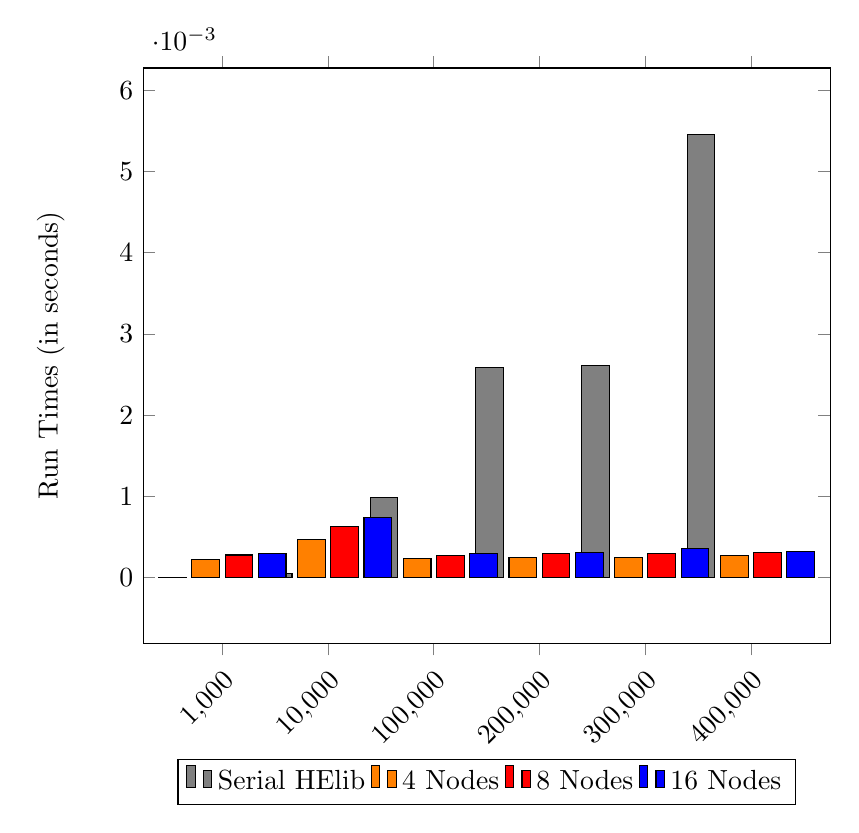
\begin{tikzpicture}

\begin{axis}[
    ybar,
    width=.85\textwidth,
    enlargelimits=0.15,
    legend style={at={(0.5,-0.2)},anchor=north,legend columns=-1},
    ylabel=Run Times (in seconds),
    symbolic x coords={$1{,}000$,$10{,}000$,$100{,}000$,$200{,}000$,$300{,}000$,$400{,}000$},
    xtick=data,
    x tick label style={rotate=45,anchor=north east},
    y label style={at={(axis description cs:-0.1,0.5)}, anchor=south},
]

\addplot[fill=gray]
    coordinates {
    ($1{,}000$,5.000E-06)($10{,}000$,4.800E-05)($100{,}000$,9.873E-04)($200{,}000$,2.588E-03)($300{,}000$,2.611E-03)($400{,}000$,5.457E-03) };
    
\addplot[fill=orange]
    coordinates {
    ($1{,}000$,2.240E-04)($10{,}000$,4.638E-04)($100{,}000$,2.373E-04)($200{,}000$,2.500E-04)($300{,}000$,2.438E-04)($400{,}000$,2.698E-04) };
    
\addplot[fill=red]
    coordinates {
    ($1{,}000$,2.773E-04)($10{,}000$,6.288E-04)($100{,}000$,2.740E-04)($200{,}000$,2.978E-04)($300{,}000$,2.913E-04)($400{,}000$,3.055E-04) };
    
\addplot[fill=blue]
    coordinates {
    ($1{,}000$,2.985E-04)($10{,}000$,7.418E-04)($100{,}000$,2.923E-04)($200{,}000$,3.083E-04)($300{,}000$,3.515E-04)($400{,}000$,3.235E-04) };
    
\legend{Serial HElib,4 Nodes,8 Nodes, 16 Nodes}
\end{axis}
\end{tikzpicture}

\caption{Add Third Level Run Times Comparison - Distribute}
\label{fig:level3ComparisonSerialDistributeAddVecs1}
\end{figure}

\begin{figure}[p]
\centering
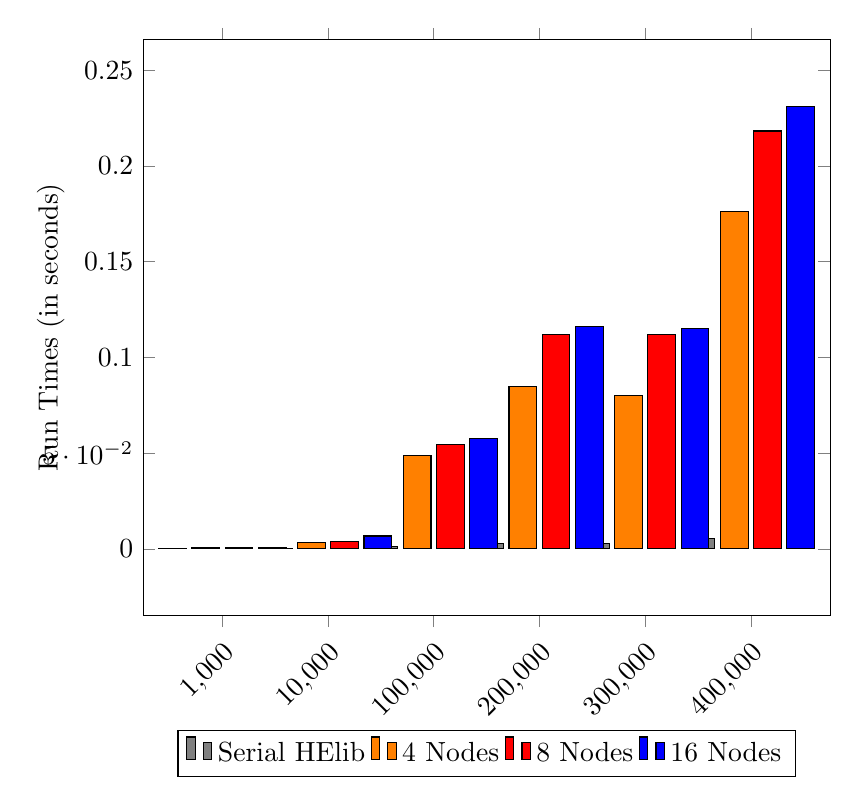
\begin{tikzpicture}

\begin{axis}[
    ybar,
    width=.85\textwidth,
    enlargelimits=0.15,
    legend style={at={(0.5,-0.2)},anchor=north,legend columns=-1},
    ylabel=Run Times (in seconds),
    symbolic x coords={$1{,}000$,$10{,}000$,$100{,}000$,$200{,}000$,$300{,}000$,$400{,}000$},
    xtick=data,
    x tick label style={rotate=45,anchor=north east},
    y label style={at={(axis description cs:-0.1,0.5)}, anchor=south},
]

\addplot[fill=gray]
    coordinates {
    ($1{,}000$,5.000E-06)($10{,}000$,4.800E-05)($100{,}000$,9.873E-04)($200{,}000$,2.588E-03)($300{,}000$,2.611E-03)($400{,}000$,5.457E-03) };
    
\addplot[fill=orange]
    coordinates {
    ($1{,}000$,5.158E-04)($10{,}000$,3.137E-03)($100{,}000$,4.874E-02)($200{,}000$,8.478E-02)($300{,}000$,8.023E-02)($400{,}000$,1.761E-01) };
    
\addplot[fill=red]
    coordinates {
    ($1{,}000$,5.903E-04)($10{,}000$,3.796E-03)($100{,}000$,5.461E-02)($200{,}000$,1.121E-01)($300{,}000$,1.122E-01)($400{,}000$,2.183E-01) };
    
\addplot[fill=blue]
    coordinates {
    ($1{,}000$,6.178E-04)($10{,}000$,6.692E-03)($100{,}000$,5.765E-02)($200{,}000$,1.163E-01)($300{,}000$,1.149E-01)($400{,}000$,2.313E-01) };
    
\legend{Serial HElib,4 Nodes, 8 Nodes, 16 Nodes}
\end{axis}
\end{tikzpicture}

\caption{Add Third Level Run Times Comparison - Sync}
\label{fig:level3ComparisonSerialDistributeAddVecs2}
\end{figure}

\begin{figure}[p]
\centering
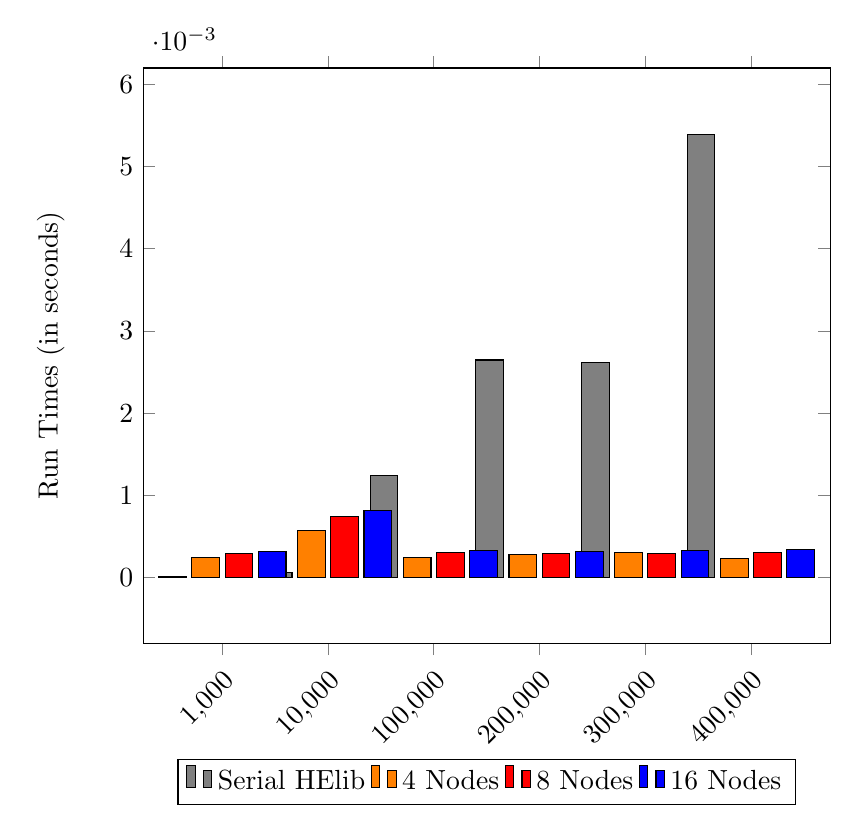
\begin{tikzpicture}

\begin{axis}[
    ybar,
    width=.85\textwidth,
    enlargelimits=0.15,
    legend style={at={(0.5,-0.2)},anchor=north,legend columns=-1},
    ylabel=Run Times (in seconds),
    symbolic x coords={$1{,}000$,$10{,}000$,$100{,}000$,$200{,}000$,$300{,}000$,$400{,}000$},
    xtick=data,
    x tick label style={rotate=45,anchor=north east},
    y label style={at={(axis description cs:-0.1,0.5)}, anchor=south},
]

\addplot[fill=gray]
    coordinates {
    ($1{,}000$,5.000E-06)($10{,}000$,5.850E-05)($100{,}000$,1.238E-03)($200{,}000$,2.646E-03)($300{,}000$,2.614E-03)($400{,}000$,5.391E-03) };
    
\addplot[fill=orange]
    coordinates {
    ($1{,}000$,2.405E-04)($10{,}000$,5.700E-04)($100{,}000$,2.470E-04)($200{,}000$,2.760E-04)($300{,}000$,2.995E-04)($400{,}000$,2.340E-04) };
    
\addplot[fill=red]
    coordinates {
    ($1{,}000$,2.915E-04)($10{,}000$,7.465E-04)($100{,}000$,3.015E-04)($200{,}000$,2.950E-04)($300{,}000$,2.955E-04)($400{,}000$,3.085E-04) };
    
\addplot[fill=blue]
    coordinates {
    ($1{,}000$,3.130E-04)($10{,}000$,8.175E-04)($100{,}000$,3.270E-04)($200{,}000$,3.190E-04)($300{,}000$,3.270E-04)($400{,}000$,3.445E-04) };
    
\legend{Serial HElib,4 Nodes,8 Nodes, 16 Nodes}
\end{axis}
\end{tikzpicture}

\caption{Sub Third Level Run Times Comparison - Distribute}
\label{fig:level3ComparisonSerialDistributeSubVecs1}
\end{figure}

\begin{figure}[p]
\centering
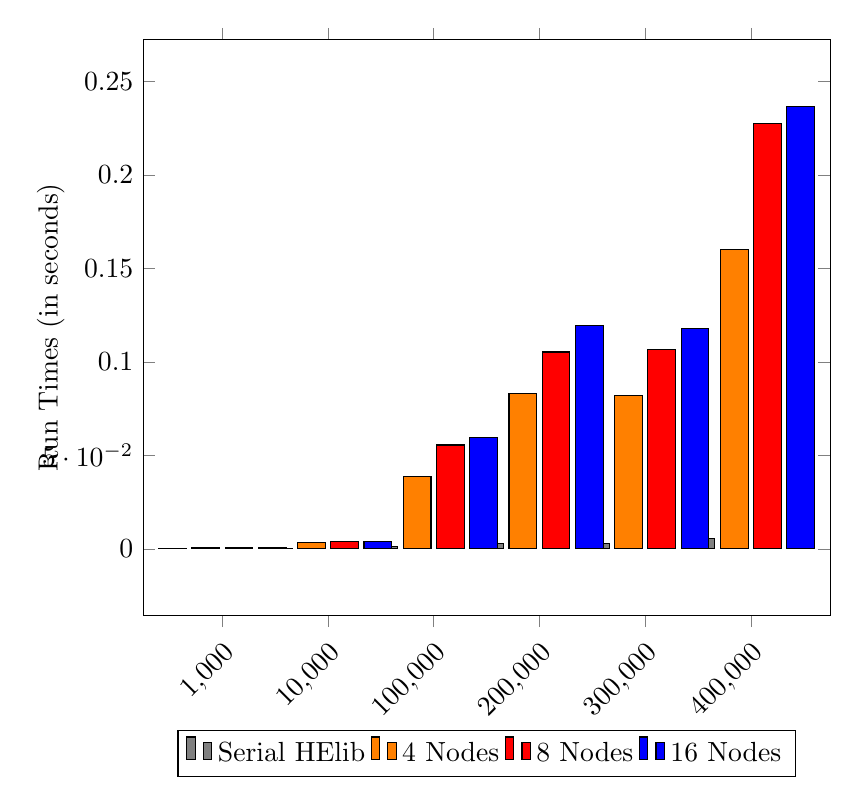
\begin{tikzpicture}

\begin{axis}[
    ybar,
    width=.85\textwidth,
    enlargelimits=0.15,
    legend style={at={(0.5,-0.2)},anchor=north,legend columns=-1},
    ylabel=Run Times (in seconds),
    symbolic x coords={$1{,}000$,$10{,}000$,$100{,}000$,$200{,}000$,$300{,}000$,$400{,}000$},
    xtick=data,
    x tick label style={rotate=45,anchor=north east},
    y label style={at={(axis description cs:-0.1,0.5)}, anchor=south},
]

\addplot[fill=gray]
    coordinates {
    ($1{,}000$,5.000E-06)($10{,}000$,5.850E-05)($100{,}000$,1.238E-03)($200{,}000$,2.646E-03)($300{,}000$,2.614E-03)($400{,}000$,5.391E-03) };
    
\addplot[fill=orange]
    coordinates {
    ($1{,}000$,5.260E-04)($10{,}000$,3.162E-03)($100{,}000$,3.861E-02)($200{,}000$,8.301E-02)($300{,}000$,8.203E-02)($400{,}000$,1.599E-01) };
    
\addplot[fill=red]
    coordinates {
    ($1{,}000$,5.940E-04)($10{,}000$,3.855E-03)($100{,}000$,5.553E-02)($200{,}000$,1.053E-01)($300{,}000$,1.066E-01)($400{,}000$,2.277E-01) };
    
\addplot[fill=blue]
    coordinates {
    ($1{,}000$,6.060E-04)($10{,}000$,4.045E-03)($100{,}000$,5.938E-02)($200{,}000$,1.196E-01)($300{,}000$,1.178E-01)($400{,}000$,2.368E-01) };
    
\legend{Serial HElib,4 Nodes, 8 Nodes, 16 Nodes}
\end{axis}
\end{tikzpicture}

\caption{Sub Third Level Run Times Comparison - Sync}
\label{fig:level3ComparisonSerialDistributeSubVecs2}
\end{figure}

\begin{figure}[p]
\centering
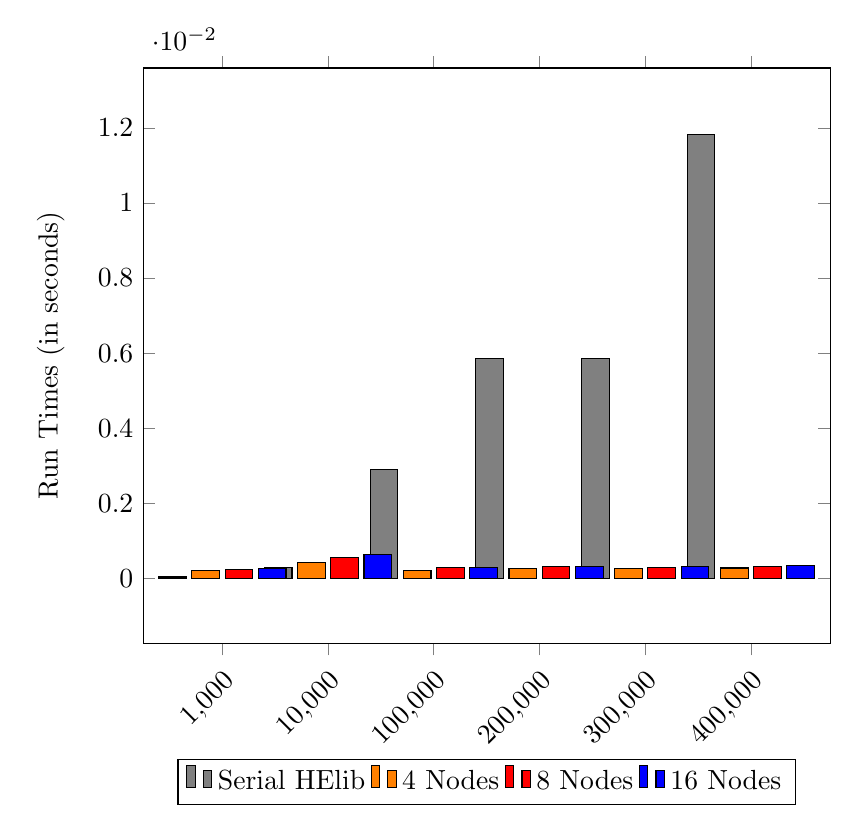
\begin{tikzpicture}

\begin{axis}[
    ybar,
    width=.85\textwidth,
    enlargelimits=0.15,
    legend style={at={(0.5,-0.2)},anchor=north,legend columns=-1},
    ylabel=Run Times (in seconds),
    symbolic x coords={$1{,}000$,$10{,}000$,$100{,}000$,$200{,}000$,$300{,}000$,$400{,}000$},
    xtick=data,
    x tick label style={rotate=45,anchor=north east},
    y label style={at={(axis description cs:-0.1,0.5)}, anchor=south},
]

\addplot[fill=gray]
    coordinates {
    ($1{,}000$,2.967E-05)($10{,}000$,2.838E-04)($100{,}000$,2.887E-03)($200{,}000$,5.845E-03)($300{,}000$,5.850E-03)($400{,}000$,1.183E-02) };
    
\addplot[fill=orange]
    coordinates {
    ($1{,}000$,2.015E-04)($10{,}000$,4.190E-04)($100{,}000$,2.150E-04)($200{,}000$,2.585E-04)($300{,}000$,2.668E-04)($400{,}000$,2.700E-04) };
    
\addplot[fill=red]
    coordinates {
    ($1{,}000$,2.427E-04)($10{,}000$,5.405E-04)($100{,}000$,2.872E-04)($200{,}000$,3.077E-04)($300{,}000$,2.953E-04)($400{,}000$,3.198E-04) };
    
\addplot[fill=blue]
    coordinates {
    ($1{,}000$,2.548E-04)($10{,}000$,6.265E-04)($100{,}000$,2.853E-04)($200{,}000$,3.130E-04)($300{,}000$,3.157E-04)($400{,}000$,3.338E-04) };
    
\legend{Serial HElib,4 Nodes,8 Nodes, 16 Nodes}
\end{axis}
\end{tikzpicture}

\caption{Mul Third Level Run Times Comparison - Distribute}
\label{fig:level3ComparisonSerialDistributeMulVecs1}
\end{figure}

\begin{figure}[p]
\centering
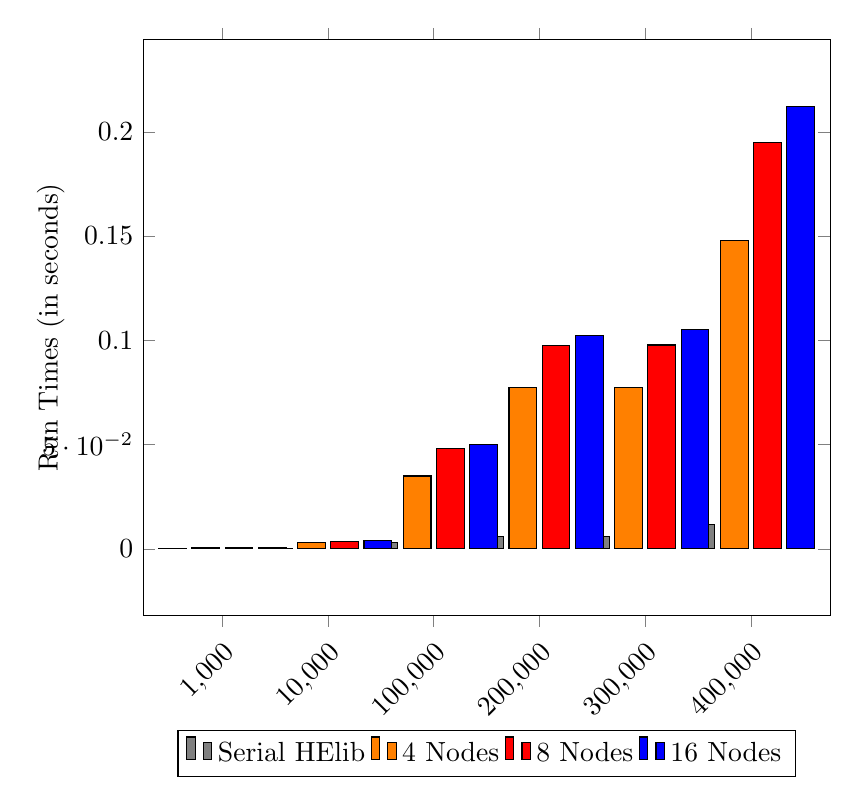
\begin{tikzpicture}

\begin{axis}[
    ybar,
    width=.85\textwidth,
    enlargelimits=0.15,
    legend style={at={(0.5,-0.2)},anchor=north,legend columns=-1},
    ylabel=Run Times (in seconds),
    symbolic x coords={$1{,}000$,$10{,}000$,$100{,}000$,$200{,}000$,$300{,}000$,$400{,}000$},
    xtick=data,
    x tick label style={rotate=45,anchor=north east},
    y label style={at={(axis description cs:-0.1,0.5)}, anchor=south},
]

\addplot[fill=gray]
    coordinates {
    ($1{,}000$,2.967E-05)($10{,}000$,2.838E-04)($100{,}000$,2.887E-03)($200{,}000$,5.845E-03)($300{,}000$,5.850E-03)($400{,}000$,1.183E-02) };
    
\addplot[fill=orange]
    coordinates {
    ($1{,}000$,5.110E-04)($10{,}000$,2.875E-03)($100{,}000$,3.495E-02)($200{,}000$,7.733E-02)($300{,}000$,7.744E-02)($400{,}000$,1.479E-01) };
    
\addplot[fill=red]
    coordinates {
    ($1{,}000$,5.608E-04)($10{,}000$,3.490E-03)($100{,}000$,4.801E-02)($200{,}000$,9.767E-02)($300{,}000$,9.774E-02)($400{,}000$,1.948E-01) };
    
\addplot[fill=blue]
    coordinates {
    ($1{,}000$,5.807E-04)($10{,}000$,3.869E-03)($100{,}000$,5.007E-02)($200{,}000$,1.022E-01)($300{,}000$,1.051E-01)($400{,}000$,2.123E-01) };
    
\legend{Serial HElib,4 Nodes, 8 Nodes, 16 Nodes}
\end{axis}
\end{tikzpicture}

\caption{Mul Third Level Run Times Comparison - Sync}
\label{fig:level3ComparisonSerialDistributeMulVecs2}
\end{figure}

Table \ref{tab:DistributedLevel3RuntimesDistribute4Nodes}, Table \ref{tab:DistributedLevel3RuntimesDistribute8Nodes}, and Table \ref{tab:DistributedLevel3RuntimesDistribute16Nodes} display the distribute run times for each operation across the three cluster sizes. Table \ref{tab:DistributedLevel3RuntimesSync4Nodes}, Table \ref{tab:DistributedLevel3RuntimesSync8Nodes}, and Table \ref{tab:DistributedLevel3RuntimesSync16Nodes} display the sync run times for each operation across the three cluster sizes. These times have been split into two plots for each operation. One group of plots focuses on the distribute times (the time it took to partition the data and assign the work) and compares them to the overall run time of the serial version. These are the \say{Distribute} plots, Figure \ref{fig:level3ComparisonSerialDistributeAddVecs1}, Figure \ref{fig:level3ComparisonSerialDistributeSubVecs1}, and Figure \ref{fig:level3ComparisonSerialDistributeMulVecs1}. The second group of plots display the sync time (the time the compute nodes took to receive the data, compute the results, and send the data back to the dispatcher node) compared to the overall run time for the serial design. Figure \ref{fig:level3ComparisonSerialDistributeAddVecs2}, Figure \ref{fig:level3ComparisonSerialDistributeSubVecs2}, and Figure \ref{fig:level3ComparisonSerialDistributeMulVecs2} display these results, and are the \say{Sync} plots.

By looking at the \say{Distribute} plots, one can see that the partitioning of data and assignment of work times across all clusters sizes and operations remains constant even when the input sizes are increased. This looks good, but remember that this part of the work only records the times it takes to partition the data and assign the work, not send the data to the compute nodes. Only non-blocking sends and receives are scheduled during this portion of the recording. The actual sending and receiving between the dispatcher and compute nodes happens mostly during the sync portion of the recording. This is because the non-blocking send and receive functions only schedule requests, which are later fulfilled in the background, during the sync part. So it is to be expected that these results are seen.

The \say{Sync} plots show where this design is failing. The amount of time needed to send the data over the network to the compute nodes, have them perform the operation and then send the data back is much greater than the serial times. This has to do with the network speed, which causes a bottleneck, and which is responsible for the plateau characteristic seen in the circuit and function level times. The network speeds are much to slow in this environment to allow for this design to be viable. With better speeds, ones which did not cause this bottleneck to happen, this design might provide better results. Additionally, future work to try and minimize the amount of data transfers between the dispatcher and compute nodes could also lead to better run times.

\section{Evaluation Conclusions} \label{sec:EvaluationConclusions}
As mentioned in the introduction of this chapter, when working with distributed systems, the overhead time, which comes from the memory transfer phases of each design, usually is the downfall of distributed systems. The same is true for these designs as well. GPUHElib suffered from slow transfer times between the CPU and GPU, which caused slow downs compared to the serial version. Similarly, DistributedHElib suffered from slow network speeds, which caused a bottleneck when transferring data between the dispatcher node and the compute nodes. With better transfer speeds, both of these designs might be viable, however under these circumstances, they are not.
\chapter{Related Work}
\chapter{Future Work} \label{chap:FutureWork}
\section{GPUHElib Future Work} \label{sec:GPUHElibFutureWork}
As seen in Chapter \ref{chap:Evaluation}, GPUHElib failed to provide any speed up over serial HElib. This was because the memory transfer times between the CPU and GPU where much too great. Therefore all of the future work for GPUHElib is designed around trying to reduce these times.

\subsection{Persistent Memory in GPU}
To cut down on memory transfer times, it would be useful to keep all the memory that needs to be transferred in the current design, in the GPUs memory permanently. Thus when the operations need to be performed, the data does not need to be transferred from the CPU to the GPU, as the GPU already contains all the data that needs to be operated on. This would reduce the memory transfer times down to almost zero, thus making the run times only dependent on the operation times, which as seen in Section \ref{sec:GPUHElibEvaluationResults}, were much lower than the serial HElib run times.

\subsection{Full Operation Implementation}
Only the most used operations were implemented on the GPU. Because of this, the results from the GPU operations needed to be copied back to the CPU, so that other unsupported operation could take place. It would be beneficial then to implement all of the operations supported by serial HElib using the GPU. Thus the results would not need to be copied back, as all the operations that a user could perform would be supported on the GPU.

\section{DistributedHElib Future Work} \label{sec:DistributedHElibFutureWork}
As seen in Chapter \ref{chap:Evaluation}, DistributedHElib failed to provide any run time improvement over serial HElib. This was a result of the network speed being a bottleneck. Thus all future work for DistributedHElib would try to reduce amount of data sent over the network.

\subsection{Distributed Memory on Compute Nodes}
In order to rely less on the network to transfer data, one could design the system so that the data is partitioned onto compute nodes. Thus each compute node would be responsible for a piece that only they were responsible for. Then when operations occur, these compute nodes can perform the operation on their piece of the data, without needing to receive the data from the dispatcher node, as the data will already be present on them. Thus data transfers would only happen during initial setup, and finalization, reducing the network traffic, and removing the network bottleneck.

\subsection{Full Operation Implementation}
Similar to the future work for GPUHElib, it would be useful to have all the operations supported on the compute nodes. Because they are not supported in the library as it is designed now, the results of operations must be sent back to the dispatcher node, so that it can perform one of these unsupported operations. With all operations supported however, the data would not need to be sent back to the dispatcher node to perform the operation, because the operation could be run on the compute nodes.
\chapter{Conclusions}
\openup -1em

\clearpage
\begin{flushleft}
\nocite{*}
\bibliography{bibliography}
\bibliographystyle{plain}
\end{flushleft}

\begin{appendices}


\end{appendices}

\end{document}
